\documentclass[
  pagePreset=smallpage,
  babelLanguage=british,
]{aruno-anecdote}

\title{Recollections of Ajahn Chah}
\subtitle{}
\author{}
\date{2013-05-03}
\ISBN{978-1-870205-65-8}
\editionInfo{\textit{Second edition}, 8,600 copies, \the\year, Printed in Malaysia}

\usepackage{mylayout}

\begin{document}

%% Frontmatter
%% ===========

\frontmatter

%% Title page
%% ----------
%% subtitle, editor, translator, preface by, introduction by, publisher

\cleartorecto
\thispagestyle{empty}

\thispagestyle{empty}

\vspace*{5em}

{\raggedleft

\begin{minipage}{0.7\textwidth}
\partTitleFont\Huge RECOLLECTIONS OF\\
\color[gray]{0.6}\textbf{AJAHN CHAH}
\end{minipage}

}



%% Copyright page
%% --------------
%% publisher info, edition info, ISBN, etc.

\cleartoverso
\thispagestyle{empty}

\thispagestyle{empty}

{\small\setlength{\parskip}{0.8em}\setlength{\parindent}{0em}%
{\raggedright%

\thetitle

For Free Distribution\\
\emph{Sabbadānaṃ dhammadānaṃ jināti}\\
The gift of the Dhamma surpasses all other gifts.

Published by Amaravati Publications,\\
Amaravati Buddhist Monastery,\\
Hertfordshire, Great Britain\\
abmpublications@amaravati.org\\
\href{http://amaravati.org}{www.amaravati.org}

Produced by Aruno Publications,\\
Aruna Ratanagiri Buddhist Monastery,\\
Northumberland, Great Britain\\
\href{http://ratanagiri.org.uk/}{www.ratanagiri.org.uk}

This book is available for free download at\\
\href{http://forestsanghabooks.org/}{www.forestsanghabooks.org}

ISBN \theISBN

Copyright \copyright\ \the\year\ AMARAVATI PUBLICATIONS

Cover design by Nicholas Halliday

\vfill

{\footnotesize
If you are interested in translating this text into another language, please contact us at abmpublications@amaravati.org

This work is licensed under a Creative Commons Attribution-NonCommercial-NoDerivs 3.0 Unported Licence.\\
\href{http://creativecommons.org/licenses/by-nc-nd/3.0/}{http://creativecommons.org/licenses/by-nc-nd/3.0/}

See page \pageref{copyright-details} for more details on your rights and restrictions under this licence.

Produced with the {\fontfamily{cms}\selectfont\LaTeX} typesetting system. Typeset in Gentium, distributed by SIL International, and Crimson Text, by Sebastian Kosch.

\theEditionInfo

}

}}



%% Acknowledgements
%% ----------------
%% * acknowledgement of sponsors

\cleartorecto
\thispagestyle{empty}

\vspace*{4\baselineskip}

{\centering

\begin{minipage}{0.9\linewidth}
\centering\small
We would like to acknowledge the support of\\
many people in the preparation of this book,\\
especially that of the Kataññutā group\\
in Malaysia, Singapore and Australia\\
for bringing it into production.

\end{minipage}

}


%% Table of Contents
%% -----------------

\tableofcontents

%% Main matter
%% ===========

\mainmatter

\partNote{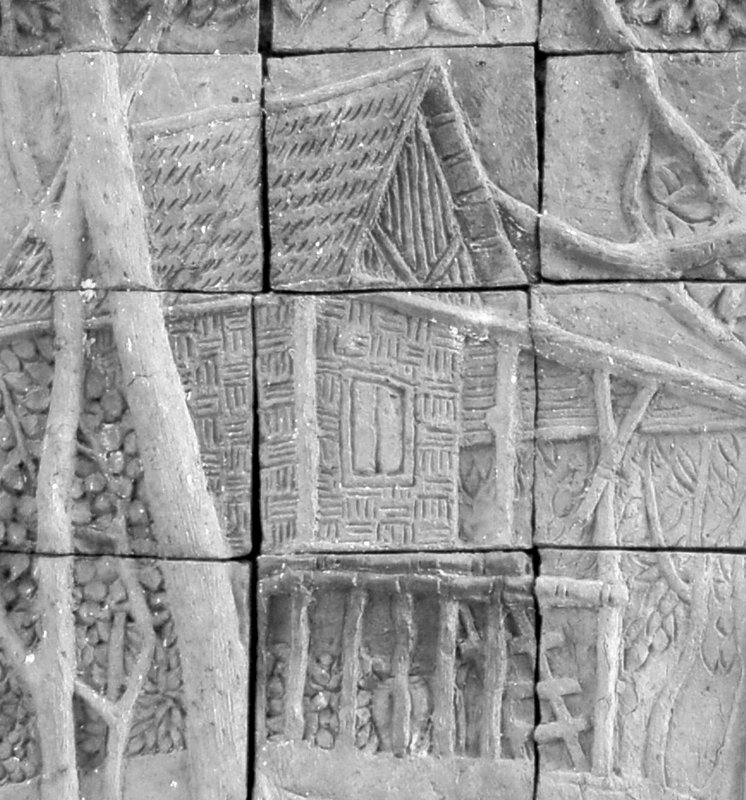
\includegraphics[keepaspectratio, width=2.8cm]{01.jpg}}
\part{Interviews with Senior Sangha Members}

\chapter{Being with Ajahn Chah}

\chapter{Being with Ajahn Chah}

\begin{quote}\itshape
The first chapter of this book has been adapted from a series of transcribed interviews which were conducted by Ajahn Kongrit Ratanawanno during his time at Amaravati Buddhist Monastery, UK. Ajahn Kongrit's home monastery is Wat Beung Saensook, Thailand. In most cases the interviewee was asked the simple question of what had inspired them most in being with Ajahn Chah.
\end{quote}

\subsection{Ajahn Sumedho}

Luang Por Chah had a great deal of \emph{mettā} (loving-kindness) and I
felt welcomed by the way he received me at Wat Pah Pong -- he seemed to
be interested in me. I felt intuitively that this was a very wise man. 
At the time I couldn't understand Thai very well, but what I saw of how
he lived his life and his general way of being was very pleasing to me. 
His teaching was very direct and he was able to see very quickly where I
was at. 

He didn't want me to spend time reading or studying, just to practise. 
He emphasized everybody's \emph{paṭipat} (practice). When I first came
to him, he told me to put my books away and to just read the
\emph{citta}, my mind. I was happy to do that, because I was weary of
studying Buddhism and wanted to practise it instead of just reading
about it. This was what he was encouraging me to do. 

Though he gave a lot of talks, which I couldn't properly understand for
the first two years, he emphasized \emph{kor wat} (monastic duties), the
way you live in the monastery: paying attention, being mindful with food
and the robes, and with the \emph{kuṭī} (hut) and the monastery. He was
like a mirror that would reflect my state of mind. He always seemed to
be completely present. I'd get carried away with thoughts and emotions
sometimes, but by just being around him, I found that I could suddenly
let go -- I could drop what I was holding onto without even telling him. 
His presence helped me to see what I was doing and what I was attached
to. So I decided that I would live with him as long as I could, since
such monks are hard to find. I stayed with him for ten years at Wat Pah
Pong and at various branch monasteries. 

\subsection{Ajahn Pasanno}

I cannot say there is really any single thing that impressed me most, 
there were many things that impressed me. Certainly Luang Por Chah set
an example for us in the sense that he didn't just teach from theory; 
when he taught he was always present -- he was an example of what was
skilful and beautiful. 

The images that come to mind are of Luang Por himself being a great
teacher and everybody respecting him so much. But I also remember a
senior monk coming to visit Wat Pah Pong, and Luang Por paying respects
to and looking after this monk. Seeing the teaching in action without
his `being the Teacher' really impressed me. It was a very direct
teaching on not-self and a living example of the ease and freedom that
come from penetrating not-self: neither a theory, nor a Buddhist
philosophy. That was the way he taught us: living the example, rather
than just giving us the philosophy. He had a great ability to teach and
draw people to the Dhamma by using these ordinary life situations. 

I remember one time we were coming back from \emph{piṇḍapat} (alms-round)
and I was walking along behind him. My Thai was not so good, so I
was just being respectful and walking close by him. We came in from the
back of the monastery, and as we were walking through the forest, two
lizards fell from a tree. Luang Por looked, then turned and said, `See
those lizards, they were mating. If they weren't caught in sensuality
they wouldn't have fallen and hurt themselves like this!' It was very
simple, and for a new monk a very funny and direct teaching. 

These are very real situations, very ordinary, and very to the point. 
Luang Por's ability to give examples and point to the things around us
empowered us to see Dhamma ourselves, rather than looking to scripture
or looking to him. To see that Dhamma is all around us and is something
we can see for ourselves was very empowering. It was both direct and had
that human quality. 

This `humanness' of Luang Por Chah was really quite striking. One time
he had some skin problems and I was helping him put ointment on the
inflammation. I would have to take off his \emph{sabong} (under-robe) to
spread the ointment all around his bottom, back and legs. And he asked, 
`Look at my bottom, does it look beautiful?' Then he would say, `It is
not beautiful, nobody would want it like this! Everybody who gets old, 
they all look like this.' Again, this is taking the ordinary and making
it something that allows us to relinquish, to let go. 

There was also his extraordinary generosity: his willingness to give of
himself, to give to people, his compassion. That was always very
touching. He never really put himself first. There was one year I was
living at Wat Pah Pong and acting as his attendant. I had been a monk
for many years by then and my Thai was very good, so I could understand
his teaching and what he was doing. I used to stay with him until
night-time, and put him to bed and massage him. It would be very rare
for him to go to bed before midnight, and sometimes he would be up until
1 or 2 a.m. Yet he was always willing to help people who were interested
in Dhamma; to give, to teach, to train, and never thought about keeping
anything for himself -- complete relinquishment, complete renunciation. 
It was very powerful. 

But it was very difficult to be his \emph{upatthak} (attendant)! It was
really hard work because he never had a schedule, just responding to
situations in an appropriate way. His flexibility came from generosity
and compassion, not from any logical sequence of how things should be. 
That was always very impressive. So there are many different aspects of
living with Luang Por Chah. It's difficult to pin it down to just one. 
If you ask me the same question tomorrow, different things will come to
mind. 

\subsection{Ajahn Ṭhiradhammo}

The most meaningful and impressive aspect to me was that he was a living
embodiment of the Buddha's teachings, which I had only previously read
about and understood conceptually. 

The first meaningful example was when I went to live at Wat Pah Pong. I
thought that if I was living in the monasteries under his guidance, I
should get to know who this great teacher Ajahn Chah was and what his
basic teaching was. I arrived there a month before the Rains Retreat
began, when there was a less formal schedule. Thus in the evening one of
the best learning situations was to sit at Ajahn Chah's hut and listen
to him interacting with visitors and resident monks. Since my Thai was
passable I could understand most of what was said. However, as I
listened to Ajahn Chah's advice, counsel and teachings, I began to feel
more confused about who he was and what his teaching was. I noticed that
he gave different teachings to different people, sometimes even giving
contrary advice. To me he thus came across as being inconsistent. So
what was it? Was he just putting on a front, or was he confused? This
presented something of a spiritual dilemma for me. On the one hand Ajahn
Chah was obviously an inspiring teacher, displaying considerable wisdom
and charisma. On the other hand, his teachings were not consistent with
how I thought an `enlightened being' should be. 

Then one evening as I listened to him, it suddenly occurred to me that
there was \emph{no fixed and consistent Ajahn Chah.}
Rather than being a person
with a particular teaching, he was actually just responding with
mindfulness and wisdom to whatever situation arose. His apparent
inconsistency was in effect a specific wise response to what the
particular person or situation required at that time. I had previously
been relating to Ajahn Chah as someone with a stable personality and a
set body of beliefs and views. Now it dawned on me that he was not
holding on to a fixed personality or definite views, but was the living
expression of mindfulness and wisdom. What appeared to be inconsistency
on the conventional level was in truth a relevant and immediate response
to whatever was happening at the time. To me this was a living example
of impersonality. 

Another example which was exceptionally helpful to me personally was
when I was bothered by the phenomenon of people's faces coming up in
meditation. They were not usually frightening, but just bothersome and
distracting. I wasn't sure what this meant or what caused it, and became
preoccupied with trying to understand or do something with it. 
Fortunately I was able to ask Ajahn Chah about this. He called it
`mental phenomena' and said, `Just observe it, and don't be fascinated
by it. Know it and go back to the breathing.' He explained that we can
become attracted by such things because they're new and interesting. He
said that I might either become quite excited about them, thinking I had
psychic powers like precognition, seeing the face of someone who next
day might offer food, or I might think that maybe ghosts were haunting
me. This was the best and most useful advice on the problem I had received from any
teacher, and when I could apply it, the faces eventually faded away. And
this principle has been very helpful for me in dealing with many of the
unusual phenomena which arise in spiritual practice. 

\subsection{Ajahn Sucitto}

The first time I saw Luang Por Chah was when he landed in Britain, when
he came through the arrivals at Heathrow Airport. There was a group of
us monks: Ajahn Sumedho, Ānando, Viradhammo, and myself. Ajahn Pabhākaro
was with Luang Por Chah. The first thing that I noticed about him was
that he was quite small, particularly compared with Ajahn Pabhākaro. But
he looked like a very, very big man -- he carried himself like a big
man; not aggressive, but completely confident. He looked like he had a
lot of space inside him. 

Here he was in a foreign country, he'd come from a long plane journey, 
couldn't speak the language, but he looked completely in charge and he
knew exactly where he wanted to be. He was not hurried. He was not
anxious. He was balanced in himself and looked warm and friendly -- not
in charge in a hard way, but at ease within his environment. Whenever we
came to see him, he was receptive; he knew how to receive people. He was
like your favourite uncle, as if you'd just been talking to him and
you'd known him all your life; very easy, very warm and you immediately
felt very relaxed. Normally when you meet somebody who's strange, you
think, `Better make sure everything's all right\ldots{}' But with him
you felt relaxed because there was the presence of \emph{mettā} --
immediately. This was overwhelming in some ways because usually almost
everybody takes a little bit of time before they warm up.

He stayed at the Hampstead Vihāra in London. This was just a small town
house. Compared with the big space of Wat Pah Pong it had very narrow
corridors and small rooms, and it was crowded. Yet he was comfortable
there. He had women sitting quite close to him, but it was no problem. 
People were not doing things properly according to the Thai way of doing
things -- not deliberately, but just not doing things in the proper way. 
And I could sense that some of the monks were quite anxious to make sure
it was all right, but he seemed to stay at ease. 

When people asked him questions, of course he couldn't understand their
words. So Ajahn Sumedho or Ajahn Pabhākaro would translate -- but he
kept his focus on the questioner. If somebody asked some very
complicated question -- about the Abhidhamma, for example -- he
would respond to the questioner rather than the question, saying things
like, `Thinking too much is not good for you', or, `Sometimes it's like
this and sometimes it's like that.' It was always a very simple answer
that went deeper than the question. It went straight to the heart. He
was never fooled by any of the questions; he always went straight to the
heart. He could feel where people were coming from. 

He was very kind: often humorous, but not dismissive. He never wavered
from being receptive and patient. People would be affected by that. People could feel that immediate heart
contact and the effect was amazing. Sometimes the place would be crowded
with people who'd sit there just so they could be there. They didn't
have any questions. They just wanted to be there, just to feel that
heart contact. People are usually nervous, tense and anxious, so to be
in a place where there was somebody like this, offering this ease and
clarity, was a blessing. You couldn't understand what he was saying and
you didn't have anything to ask, but still you wanted to be there. It
would go on for hours. He never seemed to change his pace. He never
hurried; he never hung back. Everything was just flowing. Never
hurrying, never stopping, and never moving back. It was always flowing
along, like still flowing water. That image is what he was like: still
flowing water. 

\subsection{Ajahn Munindo}

During the time I was with or nearby Luang Por Chah, I was aware he was
making a powerful impression on me, but it was only many years later
that I became clearer about just what it was that had been impressed
upon me. At the time of living in Thailand it was perhaps more like an
intuition of the `rightness' of staying there, even though it was
certainly not easy. 

I heard that somebody once asked Luang Por Chah, `How come, out of all
the monks in Thailand, you stand out as different?' Luang Por replied,
`I was willing to be daring. Others wouldn't dare do as I did.' I didn't
hear this exchange directly, it was reported to me later, but it had a
significant effect on my own attitude to practice. It signalled where
the priority lay. Knowing this about his attitude helped me to
understand his teachings better. 

Luang Por Chah wasn't worried about being popular or famous or rich, or
having lots of disciples. If he felt that something was right and should
be done, he would do it. Sometimes that took daring. From the stories of
his experiences in practice it was clear that he had to dare to confront
his own fears and resistances. He had to dare so as not to be
intimidated by the things that normally limit others. He had to dare to
contradict the views of others, even when they were strongly held. 

During the five years I was near him, the thing that continually
inspired me was how totally agile he was. My recollection of how he
handled situations stays with me and serves as a valuable support in
dealing with all that we have to face here in the West. I think I had
some sense of the way he just flowed, without resistance. Whether it was
important dignitaries coming to visit, or a simple villager who was
concerned about a sick water buffalo, or rich supporters from Bangkok, 
he always had the same beautiful ability to `go with it'. Sometimes he
would be surrounded by a large gathering of monks hanging on his every
word, and at other times he might just be sitting on his own with one or
two young monks, chewing betel nut and drinking coca cola. He was always
able to adjust without stress. There were none of the tell-tale signs of
clinging which produce suffering in an individual and generate an
atmosphere of artificiality. He was as natural as I could wish a human
being to be. I don't think I have ever seen anyone so thoroughly normal. 
Luang Por was at home wherever he went, whatever he did. He could be
quiet and sensitive when you went to see him about some personal
struggle, and a few minutes later he would be shouting orders at the
huge crowd of soldiers who had come to help build his new temple. 

This teaching example identified for me how much resistance I still had, 
and that this struggling `for' and `against' life was the source of the
problem. Sometimes we think our difficulties are caused by external
circumstances, but usually the biggest cause is our inner habits of
clinging. Luang Por didn't show any signs of resistance and accordingly
didn't manifest suffering. This state of non-suffering was real for him, 
and it was remarkable how evident it also was outwardly. Because he had
settled the great questions in his own heart, he was a catalyst for
harmony and well-being in the outer world. To have had the good fortune
to witness that was a blessing. 

\subsection{Ajahn Amaro}

One of the most impressive things about Luang Por Chah was the way that
he could display authority without being authoritarian. He was a very
good leader but not someone who had to dominate people. I didn't live
with him for a long time, and maybe the very first time I had an
exchange with him was in about April or May 1978, when I was an
\emph{anāgārika} (postulant) and Luang Por was staying with us at Wat
Pah Nanachat. As an \emph{anāgārika} I was the attendant to Ajahn
Pabhākaro, who was the abbot of the monastery. So it was my job to get
his robes and bowl ready for \emph{piṇḍapat} in the morning. I never
found it easy to get up early in the morning; I still don't. Morning is
not my best time -- I can do it as an act of will, but I have to make
the effort. 

On this particular morning I woke up and saw light coming through the
gaps between the planks of the walls. I thought, `Wow, the moon is
really bright tonight.' Then I looked at the clock and saw that it must
have stopped, and I realized, `That's not the moon; that's the sun.' So
I leapt up, threw my clothes on and raced down the path. When I got to
the back of the \emph{sāla} (main hall), all the other people had
already gone out for \emph{piṇḍapat}, but Ajahn Pabhākaro and Luang Por, 
who were going out on a nearby \emph{piṇḍapat}, still hadn't left. I
thought, `OK, I've still got time. Maybe they didn't notice.' I then
realized it was twenty-five past and they were going to leave at
half-past. So I got their robes, hoping they hadn't noticed I'd arrived
late and had missed the morning chanting and sitting. While I was down
by Ajahn Chah's feet tying up the bottom end of his robes, he said
something in Thai which I couldn't understand. I looked up slightly
anxiously at Ajahn Pabhākaro for translation. Ajahn Chah had a big grin
on his face, an incredibly friendly, loving smile. Then Ajahn Pabhākaro
translated, `Sleep is delicious.' That was the first time in my life
when I did something wrong, but instead of being criticized or punished
was met by an extraordinarily loving attitude. It was at that point that
something in my heart knew Buddhism was really very different from
anything I had encountered previously. 

Luang Por was also very flexible. He had no respect for time. And he
didn't have any respect for logical consistency. He could change his
mind or his approach in a finger-snap. A couple of years later, when
Ajahn Sumedho was starting up Chithurst monastery, I was thinking of
going back to England to visit my family. I got a telegram saying my
father was very ill with a heart attack, so I came down from Roi-Et and
then to Wat Pah Pong to pay respects to Luang Por and ask his advice. I
felt I should leave for England soon, but my question was how I should
go about this. My Thai was pretty poor, and on that occasion Ajahn
Jāgaro was translating. I explained to Luang Por that I only had one
Rains Retreat as a monk and that I was from England; my family lived
quite near Chithurst and my father had just had a heart attack and was
very sick, and what did Luang Por think I should do?

He spoke for about twenty minutes -- it was a long speech and I didn't
really catch much of it. At the end, Ajahn Jāgaro said, `Well, he said
four things. 

`\thinspace ``Go to England and when your visit to your family is finished, go and
pay your respects to Ajahn Sumedho and then come straight back to
Thailand.

`\thinspace ``Go to England and stay with your family and when your business with
your family is finished, go to stay with Ajahn Sumedho for a year and
then after that year you should come back to Thailand.

`\thinspace ``Go to England, stay with your family, when your business with your
family is finished, go stay with Ajahn Sumedho and help him out. If it
gets too difficult, you can come back to Thailand if you really want
to.

`\thinspace ``Go to England, when the business with the family is finished, go
and stay with Ajahn Sumedho and don't come back.''\thinspace '

The whole talk was delivered with exactly the same expression. It wasn't
as if any one option was preferable. As he was speaking, each single
option was an absolutely sincere piece of advice, a directive: `Do this. 
These are your instructions. Follow them to the letter!' And he wasn't
trying to be clever. It was obvious that he was being absolutely
straightforward.

Related to that was his quality of being transparent as a person. 
Someone once asked me to take a message to him, saying that some people
had just arrived at the \emph{sāla} and could he come to meet them. So I went
to his \emph{kuṭī}, where he was sitting on his rattan bench with his
eyes closed. There was no one else around. I went up and knelt in front
of him and he didn't open his eyes. So I waited a few minutes, wondering
what to do, but he still didn't open his eyes. So I said (in Thai), 
`Excuse me, Luang Por' and he opened his eyes. But it was as if there
was absolutely nobody there. He wasn't asleep; his eyes opened, but
there was no expression on his face. It was completely empty. He looked
at me, and I looked at him and said, `Luang Por, Ajahn Chu asked me to
bring a message that some people have come to the \emph{sāla} and would
it be possible for you to come and receive them?'

Again for a moment there was no expression, just this completely
spacious, empty quality on his face. Then out of nowhere, the
personality appeared. He made some remark that I didn't quite catch and
it was as if suddenly the `person' appeared; it was like watching a
being coming into existence.

There was an extraordinary quality in that
moment, seeing a being putting on a mask or a costume, as if to say, 
`OK, I'll be Ajahn Chah. I can play at being Ajahn Chah for these
people.' You could see that assumption of the personality, the body, all
the characteristics of personhood just being taken up as if he was
putting on his robe or taking up a role for the sake of emerging and
contacting other people. It was very powerful, seeing that `something'
coming out of nothing; seeing a being appearing before your eyes. 

\subsection{Ajahn Jayasāro}

I arrived at Wat Pah Pong in December 1978. It was the \emph{uposatha}
 (observance) day. I was already an \emph{anāgārika} but I hadn't shaved
my head. I had been travelling. One of the Western monks, Tan Pamutto, 
took me to his \emph{kuṭī} and shaved my head, and then we went to pay
respects to Luang Por. The moment I saw him I had a very strong feeling
that he would be my teacher, and that I didn't need to go anywhere else. 

Before I left England, Ajahn Sumedho gave me a piece of advice. He said, 
`Don't look for the perfect monastery, it doesn't exist.' Even so I got
a little side-tracked and went to stay with another teacher for a few
days. But then I came back to Wat Pah Pong and thought, `Now I can stop
travelling.'

I felt Luang Por was unlike anybody I had ever met before. I felt he was
the only totally normal person I had ever met -- everyone else was a bit
abnormal compared to him! It felt as if I'd spent my whole life
listening to people singing just a little bit out of tune, and this was
the first time I'd ever heard someone sing in tune. Or as if I'd grown
up in a country that only had plastic flowers, and then one day I
finally saw a real flower: `Ah, so that's what a real flower is. I've
only ever seen plastic flowers before.' Plastic flowers can be
beautiful, but they're nothing like real flowers.

\emph{Question:} Ajahn Chah couldn't speak English, and you, when you
came, couldn't speak Thai, so how did you learn from him?

\emph{Answer:} The teaching that you receive in a \emph{desanā} (Dhamma
talk) and in other verbal teachings is only one part of what you get
from a teacher. From the very first day, the thing that I received from
Ajahn Chah, and the thing that impressed me most, was this very strong
confidence that he was an enlightened being, and therefore that
enlightenment is real and possible. I had that belief before from books
I'd read, and to a certain extent from other teachers, but it was only
when I met Ajahn Chah that this became really grounded in my being, this
confidence that the path to Nibbāna can still be followed and that it is
possible to realize all the fruits of the Holy Life. So I was impressed
by who Ajahn Chah was, his being, as much as by his teaching. Of course
I was very inspired by his teachings, and there are many teachings that
I treasure and have made great use of in my practice.

When you become a monk, you go through periods of feeling very positive,
and you can also go through periods when you feel discouraged and very
unhappy. I think if you look closely at what sustains you when you feel
down, it's not so much the wise teachings and reflections as the faith
that what you're doing is really meaningful, and that the path of
practice does lead to Nibbāna. I've never had any disrobing doubts since
I became a monk. Other monks who understood or studied the teachings
more than I have disrobed. It didn't help them. But because I had the
presence of Ajahn Chah and afterwards the memory of Ajahn Chah, it
seemed to me there's no alternative, there's nothing else that makes
sense except to be a monk and to follow this path.

I also loved his being and how he expressed himself, his voice. If you
gave Ajahn Chah a newspaper to read out loud, or if he were just to read
names from a telephone directory, I could still listen to him for hours.

\subsection{Ajahn Khemanando}

Most of my own personal experience of Ajahn Chah comes from the period, 
beginning in January 1979, when I came to stay at Wat Pah Pong as a
layman, followed by many months as an \emph{anāgārika} or \emph{pa-khao}
 (postulant). I was a newcomer to Thailand and monastic life, and spoke
or understood very little Thai, being quite dependent on the more senior
Western monks for translations and explanations of what was happening. 
So my impressions from that time were not so much of profound dialogues
or specific instructions on meditation, but more revelations of Ajahn
Chah's character, which would often overturn my own pre-conceptions
about the nature of an enlightened being, whilst also, sometimes
simultaneously, providing evidence that he did indeed function on quite
a different level from the people by whom he was surrounded; apparently
small incidents in which Ajahn Chah would do things that didn't need
explaining, which I was able to observe to gain some food for thought. 

Once I and a fellow \emph{pa-khao}, a New Zealander, were whiling away a
hot, steamy afternoon in idle conversation on the balcony of my
\emph{kuṭī}. At Wat Pah Pong in those days, much of the formal practice
was done as a group activity in the main hall morning and evening, while
your individual \emph{kuṭī} was kind of sacrosanct, where you could
expect to be left to your own devices most of the time. We had adjacent
\emph{kuṭīs} in a far corner of the monastery and had become friends, 
offering each other companionship and support in this way, basically
relaxing and goofing off. So you can imagine how surprised and guilty we
felt when Ajahn Chah himself suddenly appeared on the path to the
\emph{kuṭī}, calling out and beckoning with his hand! We thought we were
in for a scolding for not meditating diligently, but Ajahn Chah didn't
seem bothered at all, he wasn't telling us to stop talking, but calling
to us, `Come here, come here!'

It transpired that Ajahn Chah was taking time off from being the
resident sage of Wat Pah Pong, receiving a constant stream of visitors
at his \emph{kuṭī}, and had decided to go hunting for monitor lizards
instead! Having just spotted one in the vicinity, he had come to enlist
our help, patiently miming an explanation of how to fix a string snare
to the end of a bamboo pole. Ajahn Chah was very fond of the forest
chickens, which he would feed with rice in the area around his own
\emph{kuṭī}. He wanted to protect them from their natural enemy, the
large monitor lizards which liked to eat their eggs. 

So there followed what turned out to be a hilarious scene of two rather
clumsy, inexperienced Westerners, goaded on by an enthusiastic Ajahn
Chah, their adopted spiritual guide, thrashing around in the forest
trying to catch a big lizard -- hardly the sort of thing that I had
imagined writing home about! We were quite hopeless, of course, and
eventually gave up without catching anything, but not before having a
good laugh at ourselves. 

What struck me most about this little episode was the contrast between
Ajahn Chah the lizard hunter, displaying a very natural spontaneity and
down-to-earth, almost childlike simplicity and humour, and the
awe-inspiring formality of his role as head of a large important
monastery, which up to that point was all I had ever seen of him. This
had the effect of undermining many of my own pre-conceptions regarding
what a great enlightened teacher was supposed to be like, and helped me
to see that Ajahn Chah was actually very natural and quite funny. So I
was able to feel less intimidated and more relaxed in being around him. 

I spent the \emph{Vassa} of that year as a \emph{pa-khao} with Ajahn
Chah, when he unexpectedly decided to leave Wat Pah Pong for the
monastery in his home village, Wat Gor Nork, three kilometres away. I
was the most junior of the four foreign disciples who accompanied Ajahn
Chah at that time for what turned out to be a unique Rains Retreat. He
gave some very profound Dhamma talks during this \emph{Vassa}, in
response to specific questions by more senior Western monks who took
advantage of his increased accessibility in such a small place. Most of
this was over my head at the time as my Thai was still pretty minimal, 
and I was for the most part preoccupied with various chores: cleaning
spittoons, etc., such was my lowly position.

Ajahn Chah had come to this little monastery specifically to renovate
it, and soon set about building a new \emph{sāla}. He was often to be
seen supervising the work in progress, strutting around with his big
walking-stick, barking out comments and commands in a most imperious
manner, displaying what appeared to be dissatisfaction, irritation or
even anger. It was really quite intimidating to watch and I was starting
to get a bit put off by it all, when Ajahn Chah seemed to notice that I
was having a few doubts about this performance. He looked across at me
and by way of reassurance pointed to the centre of his chest and said, 
`Nothing here; nothing here!' I realized then that he was actually a
consummate actor and could display behaviour without being at all
affected by it. He was simply doing what was necessary to get the right
response from the village workers, who are culturally conditioned to
respond to that kind of expression of authority. Another time I
witnessed him metamorphose into a really friendly, jovial old uncle or
grandfather in response to a visiting family group -- a most saccharine
performance that at the time struck me as transparently artificial. But
on reflection I could see that it was in fact just right for those
people in that situation, and they departed happy and uplifted.

Through experiences like these I learned to let go of fixed views about
how supposedly enlightened people should or should not act. Ajahn Chah
was very skilful in adapting to circumstances for the sake of inspiring
or teaching others, and this indicated a highly developed mind. But an
unenlightened observer of such outward behaviour cannot see the true
quality of a mind like that. The purity or lack of defilement cannot be
seen directly; all that can be seen is an apparently normal person
displaying normal characteristics and reactions. So we should be very
cautious about jumping to conclusions or passing judgements based on
such superficial observations. As the Buddha pointed out, it is very
difficult for an unenlightened person to know the quality of a wise
person. It needs keen observation over a long period of time -- a very
important point.

Visiting Ajahn Chah back at Wat Pah Pong after that \emph{Vassa}, I
found him directing a contingent of young conscript soldiers who had
come to help clean up the monastery, sweeping, picking up leaves, etc.
There he was, sitting in his wicker chair, waving his stick and
bellowing orders left, right and centre. Seeing it was me who had come
to sit beside him under his \emph{kuṭī}, he made an oblique reference to
the previous encounter at Wat Gor Nork by leaning over and saying with a
little grin, `You can't talk to Westerners like that, can you?'

I was impressed by how much he seemed to understand the character of
Westerners and the problems they had in undertaking the monastic
training. Although he spoke most of the time in the appropriate way for
Thais -- who are conditioned to respond to authority like that -- yet he
was adaptable and quick enough to pick up the ways of dealing with
Westerners, even those who couldn't understand his language. The
villagers were always amazed by how Ajahn Chah, who had very little in
the way of formal education or worldly sophistication, could actually
teach so many Western disciples without even speaking English. Ajahn
Chah would simply point out that they themselves were raising chickens
and buffalo all the time without knowing their language, and were
managing all right!

He was very observant and could quite accurately assess the personality
of approaching newcomers by watching their faces, their postures, the
way they walked, etc. Before they had even sat down or said anything,
Ajahn Chah would make a remark to those present, such as, `This one's
full of doubt!' which subsequent conversation would reveal to be true.

More than anything else, I think it was probably his humour that made
him attractive to Westerners, for whom conceit, views and attachment to
all sorts of worldly knowledge and sophistication could be serious
obstructions. But Ajahn Chah would have means of deflating all that in a
humorous way. It's very difficult to point out somebody's defilements in
an acceptable way that doesn't cause offence or inspire resistance or
rejection. But Westerners generally have a rather sarcastic sense of
humour, and Ajahn Chah would play on that with his own wit and make
people aware of their own faults in a very funny way, which would in
turn endear him to them even more.

Most of the time I was actually with Ajahn Chah, I didn't understand
Thai very well at all, and just as I was getting competent in the
language, he got sick and was incapacitated to the point of being unable
to speak. But although the tapes and books produced in later times made
me aware of what I had missed experiencing personally, I feel no regret
about it, because after being a monk for so many years now, I really
believe that the initiation into spiritual life of those early years
gave me something that has sustained me right up to the present.
Basically, the simple conviction that this is right; it works, it is all
you need. This conviction sprang directly from my own experience of
Ajahn Chah's example; this person who seemed to have such cast-iron
integrity, who conveyed complete certainty and a kind of natural
authority that commanded respect. Confronted almost daily by all kinds
of people, problems and questions, he was quite unshaken from this
position of inner certainty and calm. No one could upset him or make him
change his position, and this was most impressive. I had never seen
anyone so constant, and it seemed to be proof that he was operating on
quite a different level from the average person.

So although I can't really claim to have had profound discussions or a
deep, personal connection with Ajahn Chah, just the constancy of his
presence was enough to anchor me to the principles of the training he
taught. And it inspired great confidence to have an example of someone
who had achieved such results from the practice, who embodied the Dhamma
and lived it all the time. Consequently, I never really had doubts about
it or any problems in surrendering myself to it. I had never had a
teacher before or much understanding of what that might imply, and was
also a fairly critical person with a rather cynical bent. But the
example of Ajahn Chah himself made the surrender of opinions and
preferences, the endurance of simplicity and austerity, the tribulations
of diet and climate, etc. a joy to undertake.

Without such an example as a constant reminder, it's very easy to remain
stuck in one's own views and opinions, which is a major obstacle to
success in training. Westerners especially have problems because they
know so much. They know that there are other teachers, other traditions
and books all over the place, and they can just get lost, never really
grasping the point of it all. Ajahn Chah would say, `Don't read books.
Don't write home more than twice a year. You've come here to die!' The
idea of living in the forest and being simple really appealed to me, as
my character naturally disposes me to be that way. It was no great
wrench to take up the forest life.

It's often assumed that living with a teacher means having an in-depth
personal rapport, characterized by weighty discussions of profound
topics pertaining to spiritual life and the highest goals thereof. But
that's not necessarily the case. You never really enter spiritual life
whole-heartedly until you surrender yourself, surrender views and
opinions. Ajahn Chah's genius was in his ability to point this out,
orchestrating an environment or training situation in which people could
become aware of their own defilements and learn not to believe their own
thinking. This is incredibly important. Without the example of someone
who has done it; who lives it, it's really difficult to give up
self-concern. I never had any problems wondering whether I should be
doing this or whether I should go somewhere else. Inspired by Ajahn
Chah's example, I just got on with it. I didn't see any point in going
anywhere else.

Eventually you verify the teaching through your own practice, and you
realize how things change. Your habits change; your character changes.
Your defilements get less. Life gets easier and your mind is more
peaceful. Everything Ajahn Chah has been saying is true!

\subsection{Ajahn Chandapālo}

My experience with Ajahn Chah is very limited because I only saw him one
time before he got really sick, when he could still walk and talk and
function normally. While I was studying in Scotland he was invited to
visit Edinburgh, and he was with Ajahn Sumedho and Ajahn Pabhākaro. He
had just arrived that evening, and he stayed overnight and left the
following day. There was a meeting with a few people. He didn't give a
talk, just questions and answers, and I can't remember what he said, but
it did leave an impression. I remember him as someone totally at ease
and just completely normal. There was nothing really outstanding, he was
just someone who was `right there'. There was no kind of pretence or
play-acting; he was just who he was.

It was just a short meeting, a short meditation. Afterwards he answered
questions and I saw him for an hour or so. I was still quite new to
practice and Buddhism. The only monk I'd met before was Ajahn Sumedho,
so it felt like a very important and fortunate thing to be able to meet
his teacher as well. I felt very much in awe, you know -- Ajahn Chah!

We were waiting for them to arrive and I happened to be just outside in
the corridor when he came. I remember feeling quite shy and embarrassed,
not knowing how to behave. So I just raised my hands in \emph{añjalī} (a
gesture of respect) as he walked past -- he was really short and walking
with a stick. And he stopped and looked up at me, and then carried on.

\emph{Q: Do you remember what year this was in?}

\emph{A:} It must have been 1979. I remember him sitting in a chair and
just looking around, tapping things with his stick. I felt there was
kindness, a good feeling from just being in his presence. It was a long
time ago and very brief, but what stands out is that feeling of the
goodness of his presence, and that he was someone who was very much at
ease.

I've always enjoyed his teachings that have been published in books, 
like `\emph{Bodhinyana}' and `A Taste of Freedom', very inspiring.
There's an apparent simplicity in them, but also the depth and
profundity of his wisdom comes across. And even though you can read them
many times, there's still something that reaches and touches you --
something inspiring. 

\subsection{Ajahn Karuṇiko}

I met Luang Por Chah in England. He came to the Hampstead Vihāra in
1979, when I was still a layman. One of the things I noticed was just
the sense of happiness of Luang Por Chah, his joy and happiness and the
effect that had on my mind. It made me feel very happy to be around him. 
One of the most interesting things about that time was that I had been
meditating for maybe 18 months and it was very difficult, there
was pain, restlessness. But then Luang Por Chah arrived at the Vihāra, 
and my mind was very calm and peaceful. So I'd go every night because my
meditation was very good when he was there. That was very interesting --
just the power of his presence and my mind went calm. Usually it wasn't
calm, because in my early days of meditation, sitting wasn't easy. But
it was easy to sit when he was there.

Then I think just the power of his \emph{mettā} affected me -- this nice
feeling in the heart. So I really enjoyed just being around him. It was
a very special time, that week he was there; I'd go every night. It was
interesting too that even if he was downstairs in the Vihāra, still my
meditation was good, even when he was not in the room -- incredible. I
noticed that when he left to go back to Thailand. 

He used to tease people; ask people questions and tease them a little
bit. So when I sat there and I was at his feet, just in awe of this
wonderful man, he looked down at me and said, `What do you think it
would be like to sit there for one whole hour without one thought coming
into your mind?', I thought, `Oh, very enlightened!' But he said, `Like
a stone!' and I couldn't answer that! Being around him when he came to
the Hampstead Vihāra when I was a layman was a very wonderful
experience. And that's more or less the only time I really was near to
Luang Por Chah when he was well. 



\partNote{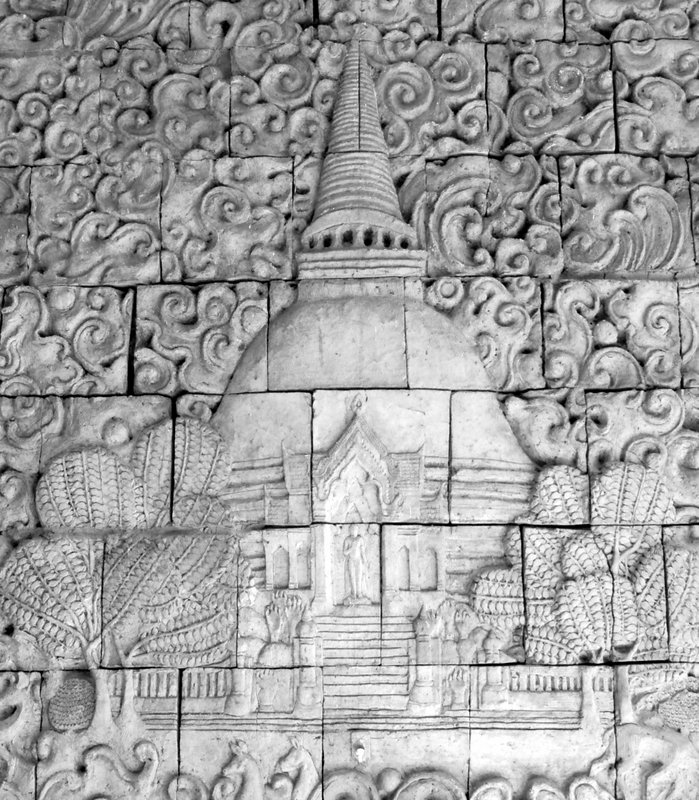
\includegraphics[keepaspectratio, width=2.8cm]{02.jpg}}
\part{Forest Sangha Newsletter Articles}

\chapterNote{Issue 9, published in July 1989.}
\chapter[Gratitude to Ajahn Chah]{Gratitude\newline \soChapter{to Ajahn Chah}}
% Title: Gratitude to Ajahn Chah
% Forest Sangha Newsletter, 1989 July.

\chapterNote{Issue 9, published in July 1989.}
\chapter[Gratitude to Ajahn Chah]{Gratitude\newline \soChapter{to Ajahn Chah}}

\begin{quote}\itshape
June 17\textsuperscript{th} was the 71\textsuperscript{st} birthday of, Venerable Ajahn Chah, spiritual
teacher of over 80 forest monasteries in Thailand, Britain and around
the world. As is customary in the monasteries in England, the day's
practice was offered in gratitude to him and for his well-being. In this
Newsletter we present, through some reflections, an occasion for readers
to recollect what he has made possible for all of us.

Venerable Jayasāro was formally abbot at Wat Pah
Nanachat. In 1988 he visited the UK as a translator for Venerable Chao
Khun Paññananda. The following reflections on Ajahn Chah's life are
taken from a talk given at Amaravati Buddhist Centre in June of that
year.
\end{quote}

\noindent
My own first meeting with Ajahn Chah was on the full moon of December
1978. I had spent the Rains Retreat of that year as an eight-precept lay
person with Ajahn Sumedho at Oakenholt in England. After the retreat I
went out to Thailand. When I arrived at Wat Pah Pong, Venerable Pamutto, 
an Australian monk resident there at the time, took me to see Ajahn
Chah. He was sitting under his \emph{kuṭī} having a drink. He looked at
me and smiled very warmly. He held out the drink he had in his hand, so
I crawled over and took it. As I returned to my place I found there were
tears welling up in my eyes. I was emotionally overcome for quite a
while. Since that day I don't think I have ever wanted to leave the
monastery or do anything except be a disciple of Ajahn Chah. 

People often presumed there would be a problem with language for
Westerners who wanted to stay at the monastery, but this was not the
case. Someone once asked Ajahn Chah: `Luang Por, how do you teach all
your Western disciples? Do you speak English or French? Do you speak
Japanese or German?' `No,' replied Ajahn Chah. `Then how do they all
manage?' he asked. `Householder', Ajahn Chah enquired, `at your home do
you have water buffaloes?' `Yes, Luang Por' was the reply. `Do you have
any cows, or dogs, or chickens?' `Yes, Luang Por.' `Tell me', Luang Por
asked, `do you speak waterbuffalo: do you speak cow?' `No,' the
householder replied. `Well, how do they all manage?'

Language was not so important to Luang Por. He knew how to see through
the exterior trappings of language and culture. He could see how all
minds basically revolve around the same old centres of greed, hatred and
delusion. His method of training was one of pointing directly at the way
our minds work. He was always showing us how craving gives rise to
suffering -- actually allowing us to see the Four Noble Truths directly.
And for him, the way of exposing desires was to frustrate them. In his
vocabulary, the words `to teach' and `to torment' were more or less
interchangeable.

Such training as this can only take place if everyone in the monastery
has great confidence in the teacher. If there is the slightest suspicion
that he might be doing it out of aversion or desire for power, there
wouldn't be any benefit. In Ajahn Chah's case everyone could see that he
had the greatest courage and fortitude, and so could trust that he was
doing it out of compassion.

Primarily he would teach about letting go. But he also taught a lot
about what to do when we can't let go. `We endure', he would say.
Usually people could appreciate intellectually about letting go, but
when faced with obstacles they couldn't do it. The teaching of patient
endurance was a central aspect of the way that he taught. He continually
changed routines around in the monastery so you wouldn't become stuck in
ruts. As a result you kept finding yourself not quite knowing where you
stood. And he would always be there watching, so you couldn't be too
heedless. This is one of the great values of living with a teacher; one
feels the need to be mindful.

In looking into Ajahn Chah's early life, it was inspiring for me to find
just how many problems he had. Biographies of some great masters leave
you with the impression that they were perfectly pure from the age
of eight or nine -- that they didn't have to work at their practice. But
for Ajahn Chah practice was very difficult. For one thing, he had a lot
of sensual desire. He also had a great deal of desire for beautiful
requisites, such as his bowl and robes, etc. He made a resolution in
working with these tendencies that he would never ask for anything, even
if it was permitted to do so by the Discipline. He related once how his
robes had been falling to bits; his under-robe was worn paper-thin, so
he had to walk very carefully lest it split. Then one day he heedlessly
squatted down and it tore completely. He didn't have any cloth to patch
it, but remembered the foot-wiping cloths in the Meeting Hall. So he
took them away, washed them and patched his robe with them.

In later times when he had disciples, he excelled in skilful means for
helping them; he had had so many problems himself. In another story, he
related how he made a resolution to really work with sensual desire. He
resolved that for the three-month Rains Retreat he would not look at a
woman. Being very strong-willed, he was able to keep to this. On the
last day of the retreat many people came to the monastery to make
offerings. He thought, `I've done it now for three months, let's see
what happens.' He looked up, and at that moment there was a young woman
right in front of him. He said the impact was like being hit by
lightning. It was then that he realized mere sense restraint, although
essential, was not enough. No matter how restrained one might be regarding
the eyes, ears, nose, tongue, body, and mind, if there wasn't wisdom to
understand the actual nature of desire, then freedom from it was
impossible.

He was always stressing the importance of wisdom, not just restraint, 
but mindfulness and contemplation. Throwing oneself into practice with
great gusto and little reflective ability may result in a strong
concentration practice, but one eventually ends up in despair. Monks
practising like this usually come to a point where they decide that they
don't have what it takes to `break through' in this lifetime, and
disrobe. He emphasized that continuous effort was much more important
than making a great effort for a short while, only to let it all slide. 
Day in, day out; month in, month out; year, in year out: that is the
real skill of the practice. 

What is needed in mindfulness practice, he taught, is a constant
awareness of what one is thinking, doing or saying. It is not a matter
of being on retreat or off retreat, or of being in a monastery or out
wandering on \emph{tudong}; it's a matter of constancy: `What am I doing
now; why am I doing it?' Constantly looking to see what is happening in
the present moment. Is this mind state coarse or refined?' At the
beginning of practice, he said, our mindfulness is intermittent, like
water dripping from a tap. But as we continue, the intervals between the
drips lessen and eventually they become a stream. This stream of
mindfulness is what we are aiming for. 

It was noticeable that he did not talk a lot about levels of
enlightenment or the various states of concentration absorption
 (\emph{jhāna}). He was aware of how people tend to attach to these terms
and conceive of practice as going from this stage to that. Once someone
asked him if such and such a person was an \emph{arahant} -- was
enlightened. He answered, `If they are then they are, if they're not, 
then they're not; you are what you are, and you're not like them. So
just do your own practice.' He was very short with such questions. 

When people asked him about his own attainments, he never spoke praising
himself or making any claim whatsoever. When talking about the
foolishness of people, he wouldn't say, `You think like this and you
think like that', or `You do this and you do that.' Rather, he would
always say, `We do this and we do that.' The skill of speaking in such a
personal manner meant that those listening regularly came away feeling
he was talking directly to them. Also, it often happened that people
would come with personal problems they wanted to discuss with him, and
that very same evening he would give a talk covering exactly that
subject. 

In setting up his monasteries, he took a lot of his ideas from the great
meditation teacher Venerable Ajahn Mun, but also from other places he
encountered during his years of wandering. Always he laid great emphasis
on a sense of community. In one section of the \emph{Mahāparinibbāna
Sutta}\footnote{Dīgha Nikāya 16.} the Buddha speaks
about the welfare of the Sangha being dependent on meeting frequently in
large numbers, in harmony, and on discussing things together. Ajahn Chah
stressed this a lot. 

The \emph{Bhikkhu} Discipline (the \emph{Vinaya}) was to Ajahn Chah a
very important tool for training. He had found it so in his own
practice. Often he would give talks on it until one or two o'clock in
the morning; the bell would then ring at three for morning chanting. 
Monks were sometimes afraid to go back to their \emph{kuṭīs} lest they
couldn't wake up, so they would just lean against a tree. 

Especially in the early days of his teaching things were very difficult. 
Even basic requisites like lanterns and torches were rare. In those days
the forest was dark and thick with many wild and dangerous animals. Late
at night you could hear the monks going back to their huts making a loud
noise, stomping and chanting at the same time, On one occasion twenty
torches were given to the monastery, but as soon as the batteries ran
out they all came back into the stores, as there were no new batteries
to replace them. 

Sometimes Ajahn Chah was very harsh on those who lived with him. He
admitted himself that he had an advantage over his disciples. He said
that when his mind entered \emph{samādhi} concentration for only 30
minutes, it could be the same as having slept all night. Sometimes he
talked for literally hours, going over and over the same things again
and again, telling the same story hundreds of times. For him, each time
was as if it was the first. He would be sitting there giggling and
chuckling away, and everybody else would be looking at the clock and
wondering when he would let them go. 

It seemed that he had a special soft spot for those who suffered a lot; 
this often meant the Western monks. There was one English monk, 
Venerable Ṭhitabho, to whom he gave a lot of attention; that means he
tormented him terribly. One day there was a large gathering of visitors
to the monastery, and as often happened, Ajahn Chah was praising the
Western monks to the Thais as a way of teaching them. He was saying how
clever the Westerners were, all the things they could do and what good
disciples they were. `All', he said, `except this one', pointing to
Venerable Ṭhitabho. `He's really stupid.' Another day he asked Venerable
Ṭhitabho, `Do you get angry when I treat you like this?' Venerable
Ṭhitabho replied, `What use would it be? It would be like getting angry
at a mountain.'

Several times people suggested to Ajahn Chah that he was like a Zen
master. `No I'm not', he would say, `I'm like Ajahn Chah.' There was a
Korean monk visiting once who liked to ask him \emph{koans}. Ajahn Chah
was completely baffled; he thought they were jokes. You could see how it
was necessary to know the rules of the game before you could give the
right answers. One day this monk told Ajahn Chah the Zen story about the
flag and the wind, and asked, `Is it the flag that blows or is it the
wind?' Ajahn Chah answered, `It's neither; it's the mind.' The Korean
monk thought that was wonderful and immediately bowed to Ajahn Chah. But
then Ajahn Chah said he'd just read the story in the Thai translation of
Hui Neng. 

Many of us tend to confuse complexity with profundity, so Ajahn Chah
liked to show how profundity was in fact simplicity. The truth of
impermanence is the most simple thing in the world, and yet it is the
most profound. He really emphasized that. He said the key to living in
the world with wisdom is a regular recollection of the changing nature
of things. `Nothing is sure,' he would constantly remind us. He was
always using this expression in Thai -- `\emph{Mai nair}!' -- meaning
`uncertain'. He said this teaching, `It's not certain', sums up all the
wisdom of Buddhism. He emphasized that in meditation, `We can't go
beyond the hindrances unless we really understand them.' This means
knowing their impermanence. 

Often he talked about `killing the defilements', and this also meant
`seeing their impermanence'. `Killing defilements' is an idiomatic
expression in the meditative Forest Tradition of north-east Thailand. It
means that by seeing with penetrative clarity the actual nature of
defilements, you go beyond them. 

While it was considered the `job' of a \emph{bhikkhu} in this tradition
to be dedicated to formal practice, that didn't mean there wasn't work
to do. When work needed doing you did it. And you didn't make a fuss. 
Work is not any different from formal practice if one knows the
principles properly. The same principles apply in both cases, as the
same body and mind are active. And in Ajahn Chah's monasteries, when the
monks worked, they really worked. One time he wanted a road built up to
Wat Tum Saeng Pet mountain monastery, and the Highways Department
offered to help. But before long they pulled out, so Ajahn Chah took the
monks up there to do it. Everybody worked from three o'clock in the
afternoon until three o'clock the next morning. A rest was allowed until
just after five, when they would head off down the hill to the village
on alms-round. After the meal they could rest again until three, before
starting work once more. But nobody saw Ajahn Chah take a rest; he was
busy receiving people who came to visit. And when it was time for work
he didn't just direct it. He joined in the heavy lifting, carrying rocks
alongside everyone else. That was always very inspiring for the monks to
see: hauling water from the well, sweeping and so on, he was always
there, right up until the time when his health began to fail. 

Ajahn Chah wasn't always popular in his province in north-east Thailand, 
even though he did bring about many major changes in the lives of the
people. There was a great deal of animism and superstition in their
belief systems. Very few people practised meditation, out of fear that
it would drive them crazy. There was more interest in magical powers and
psychic phenomena than in Buddhism. A lot of killing of animals was done
in the pursuit of merit. Ajahn Chah was often very outspoken on such
issues, so he had many enemies. 

Nevertheless, there were always many who loved him, and it was clear
that he never played on that. In fact, if any of his disciples were
getting too close, he would send them away. Sometimes monks became
attached to him, and he promptly sent them off to some other monastery. 
Charismatic as he was, he always stressed the importance of the Sangha
-- of community spirit. 

I think it was because Ajahn Chah was `nobody in particular' that he
could be anybody he chose. If he felt it was necessary to be fierce, he
could be that. If he felt that somebody would benefit from warmth and
kindness, then he would give them. You had the feeling he would be
whatever was helpful for the person he was with. And he was very clear
about the proper understanding of conventions. Someone once asked about
the relative merits of \emph{arahants} and \emph{bodhisattvas}. He
answered, `Don't be an \emph{arahant}, don't be a \emph{bodhisattva}, 
don't be anything at all. If you are an \emph{arahant} you will suffer, 
if you are a \emph{bodhisattva} you will suffer, if you are anything at
you will suffer.' I had the feeling that Ajahn Chah wasn't anything at
all. The quality in him which inspired awe was the light of Dhamma he
reflected; it wasn't exactly him as a person. 

So since first meeting Ajahn Chah, I have had an unshakeable conviction
that this way is truly possible -- it works -- it is good enough. And
I've found a willingness to acknowledge that if there are any problems, 
it's me who is creating them. It's not the form and it's not the
teachings. This appreciation made things a lot easier. It's important
that we are able to learn from all the ups and downs we have in
practice. It's important that we come to know how to be `a refuge unto
ourselves'-- to see clearly for ourselves. When I consider the morass of
selfishness and foolishness my life could have been, and then reflect on
the teachings and benefits I've received, I find I really want to
dedicate my life to being a credit to my teacher. This reflection has
been a great source of strength. This is one form of
\emph{Sanghānussati}, `recollection of the Sangha' -- recollection of
the great debt we owe our teachers. 

So I trust that you may find this is of some help in your practice.



\chapterNote{Issue 13, published in July 1990. Further recollections by those who knew him.}
\chapter{Living with Luang Por}
% Forest Sangha Newsletter, 1990 July.

\subsection{Paul Breiter}

\emph{Formerly Ven. Varapañño, writes of his early contact with Ajahn Chah (c. 1970):}

One cold afternoon as we swept the monastery grounds with long-handled
brooms, I thought how nice it would be, what a simple thing it really
was, if we could have a sweet drink of sugary coffee or tea after
working like that, to warm the bones and give us a little energy for
meditation at night. 

I had heard that Western monks in the forest tend to get infatuated with
sweets, and finally the dam burst for me. One morning on
\emph{piṇḍapat}, from the moment I walked out of the gate of the Wat to
the moment I came back about one and a half hours later, I thought
continually about sugar, candy, sweets, chocolate. Finally I sent a
letter asking a lay supporter in Bangkok to send me some palm-sugar
cakes. And I waited. The weeks went by. One day I went to town with a
layman to get medicine. We stopped by the Post Office and my
long-awaited package was there. It was huge, and ants were already at
it. 

When I got back to the Wat, I took the box to my \emph{kuṭī} and opened
it. There were 20-25 pounds of palm and sugarcane cakes. I went wild,
stuffing them down until my stomach ached. Then I thought I should share
them (otherwise I might get very sick!), so I put some aside and took
the rest to Ajahn Chah's \emph{kuṭī}. He had the bell rung, all the
monks and novices came, and everyone enjoyed a rare treat. 

That night I ate more; and the next morning I couldn't control myself. 
The sugar cakes were devouring me; my blessing started to seem like a
curse. So I took the cakes in a plastic bag and decided to go round the
monks' \emph{kuṭīs} and gave them away. 

For a start I fell down my stairs and bruised myself nicely. The wooden
stairs can get slippery in cold weather, and I wasn't being very mindful
in my guilty, distressed state of mind. 

The first \emph{kuṭī} I went to had a light on inside, but I called and
there was no answer. Finally, after I'd called several times and waited, 
the monk timidly asked who it was (I didn't yet understand how strong
fear of ghosts is among those people). I offered him some sugar, and he
asked me why I didn't want to keep it for myself. I tried to explain
about my defiled state of mind. He took one (it was hard to get them to
take much, as it is considered to be in very bad taste to display one's
desire or anger). 

I repeated this with a few others, having little chats along the way. It
was getting late, and although I hadn't unloaded all the sugar cakes, I
headed back to my \emph{kuṭī}. My flashlight batteries were almost dead, 
so I lit matches to try to have a view of the path -- there were lots of
poisonous things creeping and crawling around in the forest. I ran into
some army ants and experienced my first fiery sting. I got back to my
\emph{kuṭī} feeling very foolish. In the morning I took the rest of the
cakes and gave them to one of the senior monks, who I felt would have
the wisdom and self-discipline to be able to handle them. 

But my heart grew heavy. I went to see Ajahn Chah in the afternoon to
confess my sins. I felt like it was all over for me, there was no hope
left. He was talking with an old monk. I made the customary three
prostrations, sat down and waited. When he acknowledged me, I blurted
out, `I'm impure, my mind is soiled, I'm no good\ldots{}' He looked very
concerned. `What is it?' he asked. I told him my story. Naturally he was
amused, and within a few minutes I realized that he had me laughing. I
was very light-hearted; the world was no longer about to end. In fact, I
had forgotten about my burden. This was one of his most magical gifts. 
You could feel so burdened and depressed and hopeless, and after being
around him for a few minutes it all vanished, and you found yourself
laughing. Sometimes you only needed to go and sit down at his
\emph{kuṭī} and be around him as he spoke with others. Even when he was
away I would get a `contact high' of peacefulness as soon I got near his
\emph{kuṭī} to clean up or to sweep leaves. 

He said, `In the afternoon, when water-hauling is finished, you come
here and clean up.' My first reaction was, `He's got a lot of nerve, 
telling me to come and wait on him.' But apart from being one of my
duties, it was a foot in the door and a privilege. Through it, I was to
start seeing that there was a way of life in the monastery which is
rich, structured and harmonious. And at the centre of it all is the
teacher, who is someone to be relied on. 

Finally, he asked why I was so skinny. Immediately, one of the monks who
was there told him that I took a very small ball of rice at meal-time. 
Did I not like the food? I told him I just couldn't digest much of the
sticky rice, so I kept cutting down. I had come to accept it as the way
it was, thinking I was so greedy that eating less and less was a virtue. 
But he was concerned. Did I feel tired? Most of the time I had little
strength, I admitted. `So', he said, `I'm going to put you on a special
diet for a while -- just plain rice gruel and fish sauce to start with. 
You eat a lot of it, and your stomach will stretch out. Then we'll go to
boiled rice, and finally to sticky rice. I'm a doctor', he added. (I
found out later on that he actually was an accomplished herbalist, as
well as having knowledge of all the illnesses to which monks are prone). 
He told me not to push myself too much. If I didn't have any strength, I
didn't have to carry water, etc. 

That was when the magic really began. That was when he was no longer
just Ajahn Chah to me. He became Luang Por, `Venerable Father'. 

\subsection{Ajahn Munindo}

\emph{A visit from Luang Por:}

There was a very difficult period in my training in Thailand, after I
had already been a monk for about four years. As a result of a motorbike
accident I had had before I was ordained, and a number of years of
sitting in bad posture, my knees seized up. The doctors in Bangkok said
it was severe arthritis, but nothing that a small operation couldn't
fix. They said it would take two or three weeks. But after two months
and three operations I was still hardly walking. There had been all
kinds of complications: scar tissue, three lots of general anaesthetic
and the hot season was getting at me; my mind was really in a state. I
was thinking, `My whole life as a monk is ruined. Whoever heard of a
Buddhist monk who can't sit cross-legged?' Every time I saw somebody
sitting cross-legged I'd feel angry. I was feeling terrible, and my mind
was saying, `It shouldn't be like this; the doctor shouldn't have done
it like that; the monks' rules shouldn't be this way \ldots{}.' It was
really painful, physically and mentally. I was in a very unsatisfactory
situation. 

Then I heard that Ajahn Chah was coming down to Bangkok. I thought if I
went to see him he might be able to help in some way. His presence was
always very uplifting. When I visited him I couldn't bow properly; he
looked at me and asked, `What are you up to?' I began to complain. `Oh, 
Luang Por', I said, `It's not supposed to be this way. The doctors said
two weeks and it has been two months \ldots{}' I was really wallowing. 
With a surprised expression on his face he said to me, very powerfully, 
`What do you mean, it shouldn't be this way? If it shouldn't be
this way, it wouldn't be this way!'

That really did something to me. He pointed to exactly what I was doing
that was creating the problem. There was no question about the fact of
the pain; the problem was my denying that fact, and that was something I
was doing. This is not just a theory. When someone offers us the
reflection of exactly what we are doing, we are incredibly grateful, 
even if at that time we feel a bit of a twit. 

\subsection{Ajahn Sumedho}

\emph{An incident from his early days with Ajahn Chah (c. 1967-69):}

In those days I was a very junior monk, and one night Ajahn Chah took us
to a village fete -- I think Satimanto was there at the time. 

Now, we were all very serious practitioners and didn't want any kind of
frivolity or foolishness; so of course going to a village fete was the
last thing we wanted to do, because in these villages they love
loudspeakers. 

Anyway, Ajahn Chah took Satimanto and I to this village fete, and we had
to sit up all night with all the raucous sounds of the loudspeakers
going and monks giving talks all night long. I kept thinking, `Oh, I
want to get back to my cave. Green skin monsters and ghosts are much
better than this.' I noticed that Satimanto (who was incredibly serious) 
was looking angry and critical, and very unhappy. So we sat there
looking miserable, and I thought, `Why does Ajahn Chah bring us to these
things?' Then I began to see for myself. I remember sitting there
thinking, `Here I am getting all upset over this. Is it that bad? What's
really bad is what I'm making out of it, what's really miserable is my
mind. Loudspeakers and noise, distraction and sleepiness -- all that, 
one can really put up with. It's that awful thing in my mind that hates
it, resents it and wants to leave.'

That evening I could really see what misery I could create in my mind
over things that one can bear. I remember that as a very clear insight
of what I thought was miserable and what really is miserable. At first I
was blaming the people and the loudspeakers, and the disruption, the
noise and the discomfort, I thought that was the problem. Then I
realized that it wasn't -- it was my mind that was miserable. 

\subsection{Sister Candasiri}

\emph{Sister Candasiri first met Luang Por Chah while still a
laywoman, during his second visit to England in 1979:}

For me one of the most striking things about Luang Por Chah was the
effect of his presence on those around him. Watching Ajahn Sumedho --
who hitherto had been for me a somewhat awe-inspiring teacher -- sit at
his feet with an attitude of sheer delight, devotion and adoration
lingers in the mind as a memory of extraordinary sweetness. Ajahn Chah
would tease him, `Maybe it's time for you to come back to Thailand!'
Everyone gasped inwardly: `Is he serious?'

Later on a visitor, a professional flautist, began to ask about music.
`What about Bach? Surely there's nothing wrong with that -- much of his
music is very spiritual, not at all worldly.' (It was a question that
interested me greatly). Ajahn Chah looked at her, and when she had
finished he said quietly, `Yes, but the music of the peaceful heart is
much, much more beautiful.'

\subsection{Ajahn Santacitto}

\emph{Recollecting his own first meeting with Ajahn Chah:}

From the very first meeting with Ajahn Chah, I couldn't help but be
aware of how powerful a force was emanating from this person. I had just
arrived at the monastery with a friend, and neither of us spoke much
Thai, so the possibility of talking with and hearing Dhamma from Ajahn
Chah was very limited. I was considering taking ordination as a monk
mainly in order to learn about meditation, rather than from any serious
inclination towards religious practice. 

It happened that just at that time, a group of local villagers came to
ask him to perform a certain traditional ceremony which involved a great
deal of ritual. The laymen bowed down before the Master, then they got
completely covered over with a white cloth, and then holy water was
brought out and candles were dripped into it, while the monks did the
chanting. And young lad that I was, very science-minded, rather
iconoclastic by nature, I found this all rather startling, and wondered
just what I was letting myself in for. Did I really want to become one
of these guys and do this kind of thing? 

So I just started to look around, watching this scene unfold before me, 
until my eye caught Ajahn Chah's, and what I saw on his face was very
unexpected: there was the smile of a mischievous young man, as if he
were saying, `Good fun, isn't it!' This threw me a bit; I could no
longer think of him as being attached to this kind of ritual, and I
began to appreciate his wisdom. But a few minutes later, when the
ceremony was over and everyone got up and out from under the cloth, all
looking very happy and elated, I noticed that the expression on his face
had changed; no sign of that mischievous young lad. And although I
couldn't understand a word of Thai, I couldn't help but feel very deeply
that quality of compassion in the way he took this opportunity of
teaching people who otherwise might not have been open and susceptible. 
It was seeing how, rather than fighting and resisting social customs
with their rites and rituals, he knew how to use them skilfully to help
people. I think this is what hooked me. 

It happened countless times: people would come to the monastery with
their problems, looking for an easy answer, but somehow, whatever the
circumstances, his approach never varied. He met everybody with a
complete openness, with the `eyes of a babe', as it seemed to me, no
matter who they were. One day a very large Chinese businessman came to
visit. He did his rather disrespectful form of bowing, and as he did so
his sports shirt slipped over his back pocket, and out stuck a pistol. 
Carrying a pistol is about the grossest thing you can do when coming to
see an Ajahn in a Thai monastery! That really took me aback, but what
struck me most of all was that when Ajahn Chah looked at him, there was
that same openness, no difference, `eyes like a babe'. There was a
complete openness and willingness to go into the other person's world, 
to be there, to experience it, to share it with them. 

\subsection{Ajahn Sumedho}

\emph{Recalling an incident during Luang Por's visit to Britain in 1977:}

When Ajahn Chah first visited England, he was invited to a certain
woman's home for a vegetarian meal. She obviously had put a lot of
effort into creating the most delicious kinds of food. She was bustling
about offering this food and looking very enthusiastic. Ajahn Chah was
sitting there assessing the situation, and then suddenly he said: `This
is the most delicious and wonderful meal I have ever had!'

That comment was really something, because in Thailand, monks are not
supposed to comment on the food. And yet Luang Por suddenly manifested
this charming character in complimenting a woman who needed to be
complimented, and it made her feel so happy. He had a feeling for the
time and place, for the person he was with, for what would be kind. He
could step out of the designated role and manifest in ways that were
appropriate; he was not actually breaking any rules, but it was out of
character. Now, that shows wisdom and the ability to respond to a
situation -- not to be just rigidly bound within a convention that
blinds you. 

\subsection{Paul Breiter}

On his visit in 1979, he related that once a Westerner (a layman, I
think) came to Wat Pah Pong and asked him if he was an \emph{arahant}.
Ajahn Chah told him, `Your question is a question to be answered. I will
answer it like this: I am like a tree in the forest. Birds come to the
tree, they will sit on its branches and eat its fruit. To the birds, the
fruit may be sweet or sour or whatever. But the tree doesn't know
anything about it. The birds say `sweet' or they say `sour' -- from the
tree's point of view this is just the chattering of the birds.'

On that same evening we also discussed the relative virtues of the
\emph{arahant} and the \emph{bodhisattva}. He ended our discussion by
saying, `Don't be an arahant. Don't be a Buddha. Don't be anything at
all. Being something makes problems. So don't be anything. You don't
have to be something, he doesn't have to be something, I don't have to
be something \ldots{}' He paused, and then said, `Sometimes when I think
about it, I don't want to say anything.'



\chapterNote{Issue 20, published in April 1992. Venerable Ṭhitapañño offers an account of the events at Wat Pah Pong immediately following Luang Por Chah's death.}
\chapter{Ajahn Chah Passes Away}
% Title: Ajahn Chah Passes Away
% Forest Sangha Newsletter 1992 April

\emph{Venerable Thitapañño offers an account of the events at Wat Pah
Pong immediately following Luang Por Chah's death.}

On the morning of 16\textsuperscript{th} January, the Sangha in Britain received a brief
message from Wat Pah Nanachat to inform us of the death of Luang Por
Chah. The Venerable Ajahn had been critically ill, paralyzed and
rendered completely incapacitated by brain damage and numerous strokes
over the past ten years. Our winter retreat offered us an ideal
opportunity to pay honour to his example, reflect upon his teachings and
further our practice in the way that he made clear. 

It was during a retreat at Wat Keuan that Ajahn Sumedho and the
Western Sangha who had gathered there heard that Luang Por Chah had been
admitted to Ubon Hospital. Malfunctioning kidneys and heart
complications had proved to be beyond the medical skills of the monks
nursing him. During the ten years of his illness Luang Por had entered
hospital many times, yet on each occasion he had miraculously recovered. 
However, reports soon began to reach us that his body was refusing to
take food and the general state of his health was deteriorating. 

Early on the evening of 15th January the doctors at the ICU realized
that Luang Por's condition had deteriorated to the extent that he was
beyond medical assistance. At 10 pm Luang Por was taken by ambulance to
his nursing \emph{kuṭī} at Wat Pah Pong, in compliance with his previous
request that he might pass away in his own monastery. It was at 5.20 am
on 16th January that the body of Luang Par Chah breathed its last, and
in an atmosphere of peace the life of a great Buddhist master came to
its end. 

The attendant monks chanted the reflection that death is the natural
consequence of birth and that in the cessation of conditions is peace, 
then prepared Luang Por's body for the funeral services. As the news of
his death spread, people began to arrive to pay their respects. Soon
government officials, as representatives of the King, came to perform
the initial ceremonies necessary for a royal funeral. 

Within hours the corpse was moved to the main \emph{sāla}, where it was
laid in an ornately decorated coffin. The coffin was then sealed, and a
picture of Luang Por was placed to the left along with different
requisites such as his bowl and robes. Wreaths from the King, the Queen
and other members of the royal family were placed to the right. In front
of the coffin, extensive flower arrangements created the finishing
touches. 

As the news of Luang Por's death spread, his disciples rushed to the Wat
to pay their respects and offer their support with the preparations to
receive visitors to the monastery. It was decided that during the 15
days following Luang Por's death a Dhamma practice session would be
held, as an offering of remembrance and a focal point around which the
many incoming lay and monastic disciples could collect themselves. The
Sangha from Wat Pah Nanachat would come over every day at around 5 pm
and stay until midnight. During this period of 15 days, about 400 monks, 
70 nuns and 500 lay people resided at Wat Pah Pong, practising
meditation until midnight, listening to talks on Dhamma themes and
participating in various funeral ceremonies. Most of the Sangha were
living out under the trees of the forest, using their \emph{glot}
 (mosquito net umbrellas) as protection from the elements and insects. 
The monastery became a \emph{glot} village. 

Soon a huge open-air restaurant complex sprung up at the entrance to the
monastery, serving free food and drink to the enormous numbers of people
who began to make their way there from all over Thailand. As the days
passed, I began to feel a sense of awe as people streamed into the
monastery from early morning to late at night: people of all ages --
families, school groups and individuals. In those first few days over
50,000 books were distributed, which gives some indication of the
numbers coming. By the fourteenth and fifteenth days, the number of
people coming was steadily increasing to over 10,000 per day. As the
people entered the monastery, they filed quietly down the road leading
to the \emph{sāla}, waiting for an opportunity to enter and bow in
respect, and then to sit for a short while before making way for the
next group. Meanwhile the monks, nuns and resident laypeople would be
sitting in meditation, chanting or listening to a talk. Luang Por Jun
led the funeral chanting and various senior monks gave talks. Ajahn Mahā
Boowa, the renowned forest meditation master, came over from his own
monastery near Udorn to give a Dhamma talk, and commented on the quiet, 
harmonious atmosphere of the Wat, in contrast to the confusion and noise
he had experienced at similar funerals. 

A visit from the King's sister at this time seemed to presage the
arrival of the King for the fiftieth day ceremonies on 6\textsuperscript{th} March. As
always in Buddhism, however, especially in Thailand, nothing is certain. 
The hundredth day after the death of Luang Por will also be a day of
considerable importance. 

Because of the arrangements for the hundreds of thousands of people
expected to attend the actual burning of Luang Por's body (at similar
funerals for famous teachers, up to a million people have attended), and
also to find a day suitable for the King, it was decided to hold the
funeral early in 1993. 

For each of us Luang Por Chah has a personal meaning, depending on our
contact with him. I will always wonder and be inspired at the sight of
tens of thousands of people coming to Wat Pah Pong, to pay respects to a
person who had not spoken for ten years, and with whom most had never
had the opportunity to speak. They came to bow before the body of a
being whom they recognized as personifying our highest aspiration -- a
life free from the blindness of self-centred action. Freed of this
delusion, the goal of the Buddhist path is fulfilled. For me, the whole
occasion demonstrated the breadth and power of the influence of such a
being. 


\chapterNote{Issue 20, published in April 1992. Ven. Ñāṇavīro offers a report of the commemorative services at Wat Pah Pong fifty days after the death of Venerable Ajahn Chah.}
\chapter{The Fiftieth Day Commemoration}
% Title: The Fiftieth Day Commemoration
% Forest Sangha Newsletter 1992 April

\subsection*{Wat Pah Nanachat, 6\textsuperscript{th} March}

At 1 pm 300 laypeople and 200 monks and nuns gathered in the new
\emph{sāla}. The floor is polished granite and the walls are partially
marbled. Four huge chandeliers hang from the high ceiling. Large
garlands of flowers hang from the walls and the shrine is covered in
artificial lotuses, which look beautiful. The cry of the wild chickens
breaks into the silence -- they are all over the Wat! 

Ajahn Jun gave a \emph{desanā} at 2 p.m., mentioning the debt of gratitude we
all owe to Luang Por Chah. He exhorted us to make an effort to keep up
the practices that Luang Por Chah taught. He also talked about the
benefits of keeping good standards regarding \emph{sīla} and the monastic
conventions, and reminded us that the practice was not in the forest or
the Wat, but is the work of the mind in the body. `So all of Buddhism is
right here in this body/mind. Don't let the practice become perfunctory
-- put life into it. Even though Ajahn Chah is dead, the goodness and
virtue that he embodied are still alive.'

At 7 p.m. about 3,000 lay people and 300 monks and novices gathered in the
new sala for the evening chanting. At 9 pm Luang Por Paññananda gave a
\emph{desanā}. He started by praising Ajahn Chah as one of the great
monks of this era, who taught a pure kind of Buddhism, with nothing
extraneous. Ajahn Chah had trained a Sangha which could continue, most
notably overseas, where monasteries had arisen from his inspiration. 
They represented an historic occasion in the development of Buddhism. 

Luang Por Paññananda commented that Ajahn Chah had taught people to be
wise. The way the Pah Pong Sangha was handling the proceedings was a
good example: in Thailand some degenerate practices had crept into
funeral services, making them an excuse for a party with gambling and
alcohol. But the purpose of a funeral is for the study of Dhamma, not
for distraction! It's a lesson, a reminder. Even though Ajahn Chah is
dead, the goodness and virtue that he embodied are still alive. We must
maintain that which he gave to us all: we have to be `mediums' for Luang
Por Chah, channelling his goodness and virtue through our hearts. If we
reflect on Luang Por Chah's \emph{mettā}, \emph{sīla} and \emph{paññā}
and internalize them, then it's as if he is in our hearts, far better
than hanging a medallion with his picture on it around our necks. 

Luang Por Paññananda concluded by reflecting that the Buddha left the
Dhamma-Vinaya, not an individual, as our teacher, and that his teaching
was one of sustaining compassion, wisdom and purity. So our practice is
to wish all beings well, refraining from harming others or the
environment. Then to have wisdom -- whatever we're doing, inquiring as
to why are we doing it, what our purpose is and what is the most skilful
means. And to dwell in purity -- honouring goodness by making body, 
speech and mind good, associating with good people, and frequenting
places of goodness. 

Luang Por Paññananda had witnessed a decline in most monasteries after
the teacher died, with schisms occurring between the disciples. So we
should be careful not to get attached to views, or to wealth and gains, 
and agree to have regular meetings in order to maintain harmony. Sangha
and laity should support all the things that are in line with the way
Luang Por Chah taught, and refrain from the things he cautioned us
about. We must all help to do this. 

The evening continued with different senior monks giving talks. Ajahn
Santacitto was next, and his memory of Thai was excellent. They were
still talking when we left at 4.45 am, but probably finished at dawn
with morning \emph{pūjā}. 



\chapterNote{Issue 20, published in April 1992.}
\chapter{A Noble Life}
% Title: A Noble Life
% Forest Sangha Newsletter 1992 April

Venerable Ajahn Chah was born on 17\textsuperscript{th} June 1918 in a small village near
the town of Ubon Rajathani, north-east Thailand. Between the ages of 9
and 17 he was a \emph{sāmaṇera} (novice monk), during which time he
received his basic schooling, before returning to lay life to help his
parents on the farm. At the age of 20, however, he decided to resume
monastic life, and on April 26, 1939 he received \emph{upasampadā}
(\emph{bhikkhu} ordination).

Ajahn Chah's early monastic life followed a traditional pattern of
studying Buddhist teachings and the Pāli scriptural language. In his
fifth year his father fell seriously ill and died, a blunt reminder of
the frailty and precariousness of human life. This caused him to think
deeply about life's real purpose, for although he had studied
extensively and gained some proficiency in Pāli, he seemed no nearer to
a personal understanding of the end of suffering. Feelings of
disenchantment set in, and finally (in 1946) he abandoned his studies
and set off on mendicant pilgrimage. 

He walked some 400 km to central Thailand, sleeping in forests and
gathering alms-food in the villages on the way. He took up residence in a
monastery where the Vinaya was carefully studied and practised. While
there he was told about Venerable Ajahn Mun Bhuridatta, a most highly
respected meditation master. Keen to meet such an accomplished teacher, 
Ajahn Chah set off on foot for the north-east in search of him. 

At this time Ajahn Chah was wrestling with a crucial problem. He had
studied the teachings on morality, meditation and wisdom, which the
texts presented in minute and refined detail, but he could not see how
they could all actually be put into practice. Ajahn Mun told him that
although the teachings are indeed extensive, at their heart they are
very simple. With mindfulness established, it is seen that everything
arises in the mind; right there is the true path of practice. This
succinct and direct teaching was a revelation for Ajahn Chah, and
transformed his approach to practice. The way was clear. 

For the next seven years Ajahn Chah practised in the style of the
austere Forest Tradition, wandering through the countryside in quest of
quiet and secluded places for developing meditation. He lived in tiger-
and cobra-infested jungles, and even in charnel-grounds, using
reflections on death to overcome fear and penetrate to the true meaning
of life. In 1954, after years of wandering, he was invited back to his
home village. He settled close by, in a fever-ridden haunted forest
called `Pah Pong'. Despite the hardships of malaria, poor shelter and
sparse food, disciples gathered around him in increasing numbers. The
monastery which is now known as Wat Pah Pong began there, and eventually
branch monasteries were also established elsewhere. 

The training in Ajahn Chah's monasteries was quite strict and
forbidding. Ajahn Chah often pushed his monks to their limits, to test
their powers of endurance so that they would develop patience and
resolution. He sometimes initiated long and seemingly pointless work
projects in order to frustrate their attachment to tranquillity. The
emphasis was always on surrender to the way things are, and great stress
was placed upon strict observance of the Vinaya. 

In 1977 Ajahn Chah was invited to visit Britain by the English Sangha
Trust, a charity with the aim of establishing a locally-resident
Buddhist Sangha. He took Venerable Sumedho and Venerable Khemadhammo
along, and seeing the serious interest there, left them in London at the
Hampstead Vihāra. Another two of Ajahn Chah's Western \emph{bhikkhus}, 
who were then visiting their families in North America, were invited to
stay in London to make up a small resident Sangha. He returned to
Britain in 1979, at which time the monks were leaving London to begin
Chithurst Buddhist Monastery in Sussex. He then went on to America and
Canada to visit and teach. 

After this trip and again in 1981, Ajahn Chah spent the Rains away from
Wat Pah Pong, since his health was failing due to the debilitating
effects of diabetes. As his illness worsened, he would use his body as a
teaching, a living example of the impermanence of all things. He
constantly reminded people to endeavour to find a true refuge within
themselves, since he would not be able to teach for very much longer. 

Before the end of the 1981 Rains, he was taken to Bangkok for an
operation; however, it did little to improve his condition. Within a few
months he stopped talking, and gradually he lost control of his limbs
until he was completely paralyzed and bedridden. From then on he was
diligently nursed and attended by his \emph{bhikkhu} disciples, grateful
for the occasion to offer service to the teacher who so patiently and
compassionately showed the Way to so many. 



\chapterNote{Issue 22, published in October 1992. Extracts from a conversation between Luang Por Chah and a lay Buddhist.}
\chapter{Questions \& Answers}
% Title: Questons and Answers
% Forest Sangha Newsletter 1992 October

\chapterNote{Issue 22, published in October 1992. Extracts from a conversation between Luang Por Chah and a lay Buddhist.}
\chapter{Questions \& Answers}

\question{}
There are those periods when our hearts happen to be absorbed in
things and become blemished or darkened, but we are still aware of
ourselves, such as when some form of greed, hatred, or delusion comes
up. Although we know that these things are objectionable, we are unable
to prevent them from arising. Could it be said that even as we are aware
of them, we are providing the basis for increased clinging and
attachment, and maybe putting ourselves further back than where we
started from?

\answer{Luang Por Chah}
That's it! You must keep knowing them at that point; that's the method
of practice. I mean that simultaneously, we are both aware of them and
repelled by them, but lacking the ability to resist them; they just
burst forth.

By then it's already beyond your capability to do anything. At that
point you have to readjust yourself and then continue contemplation. 
Don't just give up on them there and then. When you see things arise in
that way you tend to get upset or feel regret, but it is possible to say
that they are uncertain and subject to change. What happens is that you
see these things are wrong, but you are still not ready or able to deal
with them. It's as if they are independent entities, the leftover kammic
tendencies that are still creating and conditioning the state of the
heart. You don't wish to allow the heart to become like that, but it
does, and it indicates that your knowledge and awareness are still
neither sufficient nor fast enough to keep abreast of things. 

You must practise and develop mindfulness as much as you can in order to
gain a greater and more penetrating awareness. Whether the heart is
soiled or blemished in some way, it doesn't matter; whatever comes up, 
you should contemplate the impermanence and uncertainty of it. By
maintaining this contemplation at each instant that something arises, 
after some time you will see the impermanence of all sense objects and
mental states. Because you see them as such, gradually they will lose
their importance, and your clinging and attachment to that which is a
blemish on the heart will continue to diminish. Whenever suffering
arises, you will be able to work through it and readjust yourself, but
you shouldn't give up on this work or set it aside. You must keep up a
continuity of effort and try to make your awareness fast enough to keep
in touch with the changing mental conditions. It could be said that so
far your development of the Path still lacks sufficient energy to
overcome the mental defilements; whenever suffering arises, the heart
becomes clouded over. But one must keep developing that knowledge and
understanding of the clouded heart; this is what you reflect on. 

You must really take hold of it and repeatedly contemplate that this
suffering and discontentment are just not sure things. They are
something that is ultimately impermanent, unsatisfactory, and not-self. 
Focusing on these three characteristics, whenever these conditions of
suffering arise again, you will know them straightaway, having
experienced them before. 

Gradually, little by little, your practice should gain momentum, and as
time passes, whatever sense objects and mental states arise will lose
their value in this way. Your heart will know them for what they are and
accordingly put them down. When you reach the point where you are able
to know things and put them down with ease, they say that the Path has
matured internally and you will have the ability to bear down swiftly
upon the defilements. From then on there will just be the arising and
passing away in this place, the same as waves striking the seashore. 
When a wave comes in and finally reaches the shoreline, it just
disintegrates and vanishes; a new wave comes and it happens again, the
wave going no further than the limit of the shoreline. In the same way, 
nothing will be able to go beyond the limits established by your own
awareness. 

That's the place where you will meet and come to understand
impermanence, unsatisfactoriness and not-self. It is there that things
will vanish -- the three characteristics of impermanence, 
unsatisfactoriness and not-self are the same as the seashore, and all
sense objects and mental states that are experienced go in the same way
as the waves. Happiness is uncertain; it's arisen many times before. 
Suffering is uncertain; it's arisen many times before. That's the way
they are. In your heart you will know that they are like that, they are
`just that much'. The heart will experience these conditions in this
way, and they will gradually keep losing their value and importance. 
This is talking about the characteristics of the heart, the way it is. 
It is the same for everybody, even the Buddha and all his disciples were
like this. 

If your practice of the Path matures, it will become automatic and it
will no longer be dependent on anything external. When a defilement
arises, you will immediately be aware of it and accordingly be able to
counteract it. However, that stage when they say that the Path is still
neither mature enough nor fast enough to overcome the defilements is
something that everybody has to experience -- it's unavoidable. But it
is at this point that you must use skilful reflection. Don't go
investigating elsewhere or trying to solve the problem at some other
place. Cure it right there. Apply the cure at that place where things
arise and pass away. Happiness arises and then passes away, doesn't it? 
Suffering arises and then passes away, doesn't it? You will continuously
be able to see the process of arising and ceasing, and see that which is
good and bad in the heart. These are phenomena that exist and are part
of nature. Don't cling tightly to them or create anything out of them at
all. 

If you have this kind of awareness, then even though you will be coming
into contact with things, there will not be any noise. In other words, 
you will see the arising and passing away of phenomena in a very natural
and ordinary way. You will just see things arise and then cease. You
will understand the process of arising and ceasing in the light of
impermanence, unsatisfactoriness, and not-self. 

The nature of the Dhamma is like this. When you can see things as `just
that much', then they will remain as `just that much.' There will be
none of that clinging or holding on -- as soon as you become aware of
attachment, it will disappear. There will be just the arising and
ceasing, and that is peaceful. That it's peaceful is not because you
don't hear anything; there is hearing, but you understand the nature of
it and don't cling or hold on to anything. This is what is meant by
peaceful -- the heart is still experiencing sense objects, but it
doesn't follow or get caught up in them. A division is made between the
heart, sense objects and the defilement; but if you understand the
process of arising and ceasing, then there is nothing that can really
arise from it -- it will end just there. 



\chapterNote{Issue 23, published in January 1993. The second in a series of extracts from a conversation between Luang Por Chah and a lay Buddhist.}
\chapter{Questions \& Answers II}
% Title: Questions and Answers II
% Forest Sangha Newsletter 1993 January

\question{}
Does one have to practise and gain \emph{samādhi} (concentration) before one
can contemplate the Dhamma?

\answer{Luang Por Chah}
We can say that's correct from one point of view,
but from the aspect of practice, \emph{paññā} has to come first. In
conventional terms, it's \emph{sīla}, \emph{samādhi} and then
\emph{paññā}, but if we are truly practising the Dhamma, then
\emph{paññā} comes first. If \emph{paññā} is there from the beginning, 
it means that we know what is right and what is wrong; and we know the
heart that is calm and the heart that is disturbed and agitated. 

Talking from the scriptural basis, one has to say that the practice of
restraint and composure will give rise to a sense of shame and fear of
any form of wrong-doing that potentially may arise. Once one has
established the fear of that which is wrong and one is no longer acting
or behaving wrongly, then that which is wrong will not be present within
one. When there is no longer anything wrong present within, this
provides the conditions from which calm will arise in its place. That
calm forms a foundation from which \emph{samādhi} will grow and develop over
time. 

When the heart is calm, that knowledge and understanding which arises
from within that calm is called \emph{vipassanā}. This means that from
moment to moment there is a knowing in accordance with the truth, and
within this are contained different properties. If one was to set them
down on paper they would be \emph{sīla}, \emph{samādhi} and
\emph{paññā}. Talking about them, one can bring them together and say
that these three dhammas form one mass and are inseparable. But if one
were to talk about them as different properties, then it would be
correct to say \emph{sīla}, \emph{samādhi} and \emph{paññā}. 

However, if one was acting in a unwholesome way, it would be impossible
for the heart to become calm. So it would be most accurate to see them
as developing together, and it would be right to say that this is the
way that the heart will become calm. Talking about the practice of
\emph{samādhi:} it involves preserving \emph{sīla}, which includes
looking after the sphere of one's bodily actions and speech, in order
not to do anything which is unwholesome or would lead one to remorse or
suffering. This provides the foundation for the practice of calm, and
once one has a foundation in calm, this in turn provides a foundation
which supports the arising of \emph{paññā}. 

In formal teaching they emphasize the importance of \emph{sīla}. 
\emph{Ādikalyānaṃ, majjhekalyānaṃ, pariyosānakalyānaṃ} -- the practice should
be beautiful in the beginning, beautiful in the middle and beautiful in
the end. This is how it is. Have you ever practised \emph{samādhi}? 

\bigskip

\noindent
I am still learning. The day after I went to see Tan Ajahn at Wat
Keu, my aunt brought a book containing some of your teaching for me
to read. That morning at work I started to read some passages which
contained questions and answers to different problems. In it you said
that the most important point was for the heart to watch over and
observe the process of cause and effect that takes place within; just to
watch and maintain the knowing of the different things that come up. 

That afternoon I was practising meditation, and during the sitting the
characteristic that appeared was that I felt as though my body had
disappeared. I was unable to feel the hands or legs and there were no
bodily sensations. I knew that the body was still there, but I couldn't
feel it. In the evening I had the opportunity to go and pay respects to
Tan Ajahn Tate, and I described to him the details of my experience. He
said that these were the characteristics of the heart that appear when
it unifies in \emph{samādhi}, and that I should continue practising. I
had this experience only once; on subsequent occasions I found that
sometimes I was unable to feel only certain areas of the body, such as
the hands, whereas in other areas there was still feeling.

\question{}
Sometimes
during my practice I start to wonder whether just sitting and allowing
the heart to let go of everything is the correct way to practise; or
else should I think over and occupy myself with the different problems
or unanswered questions concerning the Dhamma which I still have? 

\answer{Luang Por Chah}
It's not necessary to keep going over or adding anything
on at this stage. This is what Tan Ajahn Tate was referring to; one must
not repeat or add onto that which is there already. When that particular
kind of knowing is present, it means that the heart is calm and it is
that state of calm which one must observe. Whatever one feels, whether
it feels like there is a body or a self or not, this is not the
important point. It should all come within the field of one's awareness. 
These conditions indicate that the heart is calm and has unified in
\emph{samādhi}. 

When the heart has unified for a long period a few times, then there
will be a change in the conditions and they say that one `withdraws'. 
That state is called \emph{appanā samādhi} (absorption), and having
entered it, the heart will subsequently withdraw. In fact, although it
would not be incorrect to say that the heart withdraws, it doesn't
actually withdraw. Another way is to say that it flips back, or that it
changes, but the style used by most teachers is to say that once the
heart has reached the state of calm, then it will withdraw. However, 
people get caught up in disagreements over the use of language. It can
cause difficulties and one might start to wonder, `How on earth can it
withdraw? This business of withdrawing is just confusing!' It can lead
to much foolishness and misunderstanding just because of the language. 

What one must understand is that the way to practise is to observe these
conditions with \emph{sati-sampajañña} (mindfulness and clear
comprehension). In accordance with the characteristic of impermanence, 
the heart will turn about and withdraw to the level of \emph{upacāra
samādhi} (access concentration). If it withdraws to this level, one can
gain understanding through awareness of sense impressions and mental
states, because at the deeper level (where the mind is fixed with just
one object) there is no understanding. If there is awareness at this
point, that which appears will be \emph{saṅkhāra} (mental formations). 
It will be similar to two people having a conversation and discussing
the Dhamma together.

One who misunderstands this might feel disappointed
that his heart is not really calm, but in fact this dialogue takes place
within the confines of the calm and restraint which have developed. 
These are the characteristics of the heart once it has withdrawn to the
level of \emph{upacāra} -- there will be the ability to know about and
understand different things. 

The heart will stay in this state for a period and then it will turn
inwards again. In other words, it will turn and go back into the deeper
state of calm where it was before; or it is even possible that it might
obtain purer and calmer levels of concentrated energy than were
experienced before. If it does not reach such a level of concentration, 
one should merely note the fact and keep observing until the time when
the heart withdraws again. Once it has withdrawn, different problems
will arise within the heart. 

This is the point where one can have awareness and understanding of
different things. Here is where one should investigate and examine the
different preoccupations and issues which affect the heart, in order to
understand and penetrate them. Once these problems are finished with, 
the heart will gradually move inwards towards the deeper level of
concentration again. The heart will stay there and mature, freed from
any other work or external impingement. There will just be the
one-pointed knowing, and this will prepare and strengthen one's
mindfulness until the time to re-emerge is reached. 

These conditions of entering and leaving will appear in one's heart
during the practice, but this is something that is difficult to talk
about. It is not harmful or damaging to one's practice. After a period
the heart will withdraw and the inner dialogue will start in that place, 
taking the form of \emph{saṅkhāra} (mental formations) conditioning the
heart. If one doesn't know that this activity is \emph{saṅkhāra}, one
might think that it is \emph{paññā}, or that \emph{paññā} is arising. 
One must see that this activity is fashioning and conditioning the
heart, and the most important thing about it is that it is impermanent. 
One must continually keep control and not allow the heart to start
following and believing in all the different creations and stories that
it cooks up. All that is just \emph{saṅkhāra}, it doesn't become
\emph{paññā}. 

The way \emph{paññā} develops is when one listens and knows the heart
as the process of creating and conditioning takes it in different
directions, and one reflects on the instability and uncertainty of this. 
The realization of its impermanence will provide the cause by which one
can let go of things at that point. Once the heart has let go of things
and put them down at that point, it will gradually become more and more
calm and steady. One must keep entering and leaving \emph{samādhi} like
this, and \emph{paññā} will arise at that point. There one will gain
knowledge and understanding. 

As one continues to practise, many different kinds of problems and
difficulties will tend to arise in the heart; but whatever problems the
world or even the universe might bring up, one will be able to deal with
them all. One's wisdom will follow them up and find answers for every
question and doubt. Wherever one meditates, whatever thoughts come up, 
whatever happens, everything will be providing the cause for
\emph{paññā} to arise. This is a process that will take place by itself, 
free from external influence.

\emph{Paññā} will arise like this, but
when it does, one should be careful not to become deluded and see it as
\emph{saṅkhāra}. Whenever one reflects on things and sees them as
impermanent and uncertain, one shouldn't cling or attach to them in any
way. If one keeps developing this state, when \emph{paññā} is present in
the heart, it will take the place of one's normal way of thinking and
reacting, and the heart will become fuller and brighter in the centre of
everything. As this happens one knows and understands all things as they
really are -- one's heart will be able to progress with meditation in
the correct way and without being deluded. That is how it should be. 



\chapterNote{Issue 27, published in January 1994.}
\chapter{Recollections by Jack Kornfield}
% Title: Jack Kornfield
% Forest Sangha Newsletter 1994 January

\chapterNote{Issue 27, published in January 1994.}
\chapter{Recollections by Jack Kornfield}

\begin{quote}
`I was enormously blessed to meet Ajahn Sumedho in 1967 at
an old ruined Cambodian temple on a mountain-top in Sakolnakorn, 
Thailand. With his inspiration I went to see Ajahn Chah at Wat Pah Pong, 
and eventually entered as a monk in 1969. I left to come back to the USA
in 1972, and was re-ordained to live as a monk with Ajahn Chah for a
time in 1982. Like all of us who were with him, I could tell many more
wonderful stories. Most simply, Ajahn Chah was the wisest man I have ever known, and one of
the most delightful, and it has completely
changed my life to have him for a teacher.'
\end{quote}

\noindent
Ajahn Chah had four basic levels of teaching, and each one, although at
times very difficult for the students, was taught with a lot of humour
and a lot of love. Ajahn Chah taught that until we can begin to respect
ourselves and our environment, practice doesn't really develop. And that
dignity, the ground of practice, comes through surrender, through
impeccable discipline. A lot of us in the West understand freedom to
mean freedom to do what we want, but I think you can see that to follow
the wants of the mind isn't terribly free. It's actually rather
troublesome. 

A deeper freedom, taught through Dhamma, is the freedom within form: the
freedom we can find while relating to another human being, the freedom
of being born in a body with its limitations, and the freedom of a tight
monastic form. What Ajahn Chah did was create a situation of dignity and
demand. He really asked a lot from people, probably more than they'd
ever been asked in their whole life -- to give, to pay attention, to be
wholehearted. Sometimes practice is wonderful: the mind gets so clear
that you smell and taste the air in ways that you haven't since
you were a child. But sometimes it's difficult. He said, `That's not the
point; the point is somehow to come to inner freedom.'

We used to sit for long hours at times, and the meditation hall for the
monks was a stone platform -- they don't use cushions in Asia. You have a
square cloth like a handkerchief that you put down on the stone to sit
on. I remember that when I started, because sitting on the floor was so
painful, I would arrive early at the hall and get a place where I could
sit next to one of the pillars and lean against it. After about a week
of being with Ajahn Chah, he gathered the monks together for an evening
talk after the sitting, and he began to talk about how the true practice
of Dhamma was to become independent in any circumstance; not to need to
lean on things. And then he looked at me. 

Sometimes you would sit while he'd talk to someone or receive visitors, 
and you couldn't leave until you were dismissed. And you'd sit and sit, 
and you'd look at your mind, and it would go, `Doesn't he know that we
are sitting here? Doesn't he know I'm thirsty or I want to get up?' And
he'd be talking away -- he knew very well. And you'd sit and sit and
just see all the movement of the mind. We would sit for hours. The
quality of endurance in the monks' life in the forest, where you just
sit and sit and sit, is a very important one. 

He trusted that people came in order to learn and grow, and when it was
hard, that was all right by him. He didn't care if people had a hard
time. He would go up to them when they were having a hard time and he'd
say, `Are you angry? Whose fault is that, mine or yours?' So one really
had to give up a lot, but it wasn't to him or for him -- it was for
oneself. With surrender and dignity one learned to open up and see
clearly. It is essential in our practice to be unflinchingly honest
about ourselves and the world -- just as he was. 

He would sit under his \emph{kuṭī}, and various lay visitors and other
disciples would come, and also some of his monks would be sitting
around, and he would make fun of people. He'd say, `I'd like to
introduce you to my monks. This one, he likes to sleep a lot. And this
one, he is always sick, his health is his thing; he just spends his time
worrying about his health. And this one is a big eater -- he eats more
than two or three other monks. And this is a doubter over there, he
really likes to doubt, really gets into it. And can you imagine, he had
three different wives at the same time. And this one likes to sit a lot, 
all he does is go and sit in his \emph{kuṭī}; I think he is afraid of
people.' And then he'd point to himself and say, `Myself, I like to play
teacher.'

Once, when he came to the USA, there was a man who had been a monk with
him for a long time who had then disrobed and taken ordination as a Zen
priest. So he said, `I can't figure out this guy', (this man was acting
as his translator), `he is not quite a monk and he is not quite a lay
person. He must be some kind of a transvestite.' And throughout the next
ten days he kept introducing this man as Miss whatever his name was --
Frank or John: `This is Miss John. I'd like you to meet my
transvestite translator. He can't quite make up his mind.' He was very
funny, but he was unstintingly honest. He really could make people look
at themselves and their attachments. When I was translating for him, he
said, `Even though I don't speak any English, I know the truth is that
my translator leaves out all the really hard things I say. I tell you
painful things and he leaves out all the things that have a sting in
them, makes them soft and gentle for you. You can't trust him.'

First come dignity and surrender -- really seeing the power of one's
willingness to live in a full way in the Dhamma. And secondly, one has
to learn to see honestly, to be honest about oneself and the people
around one, to see one's limits and not to be caught in the things
outside. When I asked what is the biggest problem with new disciples, he
said, `Views and opinions about everything. They are all so educated. 
They think they know so much. When they come to me, how can they learn
anything? Wisdom is for you to watch and develop. Take from the teacher
what's good, but be aware of your own practice. If I am resting while
you all sit up, does it make you angry? If I say that the sky is red
instead of blue, don't follow me blindly. One of my teachers ate very
fast and made noises as he ate. Yet he told us to eat slowly and
mindfully. I used to watch him and got very upset. I suffered, but he
didn't. I watched the outside. Later, I learned. Some people drive very
fast but carefully, and others drive slowly and have many accidents. 
Don't cling to rules or to form. If you watch others at the most ten
percent of the time and yourself ninety percent, this is proper
practice. First I used to watch my teacher, Ajahn Tongrat, and had many
doubts. People even thought he was mad. He would do strange things and
be very fierce with his disciples. Outside he was angry, but inside
there was nobody, nothing there. He was remarkable. He stayed clear and
mindful until the moment he died. Looking outside of yourself is
comparing, discriminating; you won't find happiness that way. No way
will you find peace if you spend your time looking for the perfect man, 
or the perfect woman or the perfect teacher.'

The Buddha taught us to look at the Dhamma, the Truth, not to look at
other people, to see clearly and to see into ourselves; to know our
limits. Ram Dass asked him about limits. He asked, `Can you teach if
your own work isn't completed, if you're not fully enlightened?' And he
replied, `Be honest with them. Tell them what you know from your heart
and tell people what's possible. Don't pretend to be able to lift big
rocks when you can only lift small ones. Yet it doesn't hurt to tell
people that if you exercise and if you work, it's possible to lift this. 
Just be straightforward and assess what's truly reasonable.' Surrender, 
and dignity in that, and real impeccability: this is the ground. Then
there's clarity, seeing what's true in oneself, seeing one's limits, 
seeing one's attachments. 

Then the third way he taught was by working with things. 

Working is done in two parts: one by overcoming obstacles and
hindrances, and the other by letting go. Overcoming: the first Dhamma
talk I gave was at a large gathering, \emph{Māgha Pūjā} festival
day, and in a hall filled with 500 or 1,000 villagers. We sat up all
night, alternately sitting for one hour and then listening to a talk
given by one of the teachers from his monasteries. He had several
hundred monks there at that time; they all came together from the branch
monasteries for that day. And then in the middle of the night with no
preparation, he said, `Now we'll hear a Dhamma talk from the Western
monk.' I'd never given a Dhamma talk before, much less in Lao, the local
dialect. There was no time, I had to just get up and say what I could
say. He had his chief Western disciple, Ajahn Sumedho, get up and give a
talk. Ajahn Sumedho ended after an hour and Ajahn Chah said, `Talk
more.' So Ajahn Sumedho talked another half-hour; he didn't have much to
say, people were getting bored, he was getting bored, he finished. Ajahn
Chah said, `Now more.' Another half-hour, three-quarters of an hour, it
was getting more and more boring -- he'd run out of things to say. 
People were sleeping; Ajahn Sumedho didn't know what to say, finally
finished, and Ajahn Chah said, `More, a bit more.' Another half-hour
-- it was the most boring talk! And why would he do it? He got Ajahn
Sumedho to learn not to be afraid of being boring. It was wonderful. 

He encouraged people to put themselves in situations where they were
afraid. He would send people who were afraid of ghosts to sit outside at
night in the charnel-ground. I would go sometimes -- because I wasn't
afraid of ghosts, it was a way of showing off -- but for them it was
really scary. Or he had people go away out in the forest and meditate, 
and face the fear of tigers. The spirit of the practice was to really
make yourself work with things to overcome them. He pushed you into what
you disliked. If you liked to be alone in the forest, you were assigned
to a city monastery in Bangkok. And if you liked the city and the easy
life and good food, he'd send you to some impoverished forest monastery
where there were just rice and tree leaves to eat. He was a real rascal. 
He knew all of your trips, and he could find them and he would somehow, 
in a very funny and gentle and yet direct way, really make you look to
see where you were afraid or attached. Fear, boredom, restlessness --
fine, sit with it. Be bored, be restless and die, he would say over and
over again. Die in that restlessness, die in that fear, die in that
boredom. People were sleepy, great: the ascetic practice he'd assign
would be to sit up all night, and if you wouldn't sit, walk, walk more, 
walk backwards if you were really sleepy. Whatever it took, to really go
against it. 

With anger, restlessness, the same. He said, `You are restless. Fine, go
back and sit. Sit more when you are restless, don't sit less.' He said
it's like starving a tiger to death in a cage of mindfulness. It's not
that you need to do anything about the tiger -- the tiger being your
anger or restlessness -- just let it roam around in the cage. But you
make the cage around it with your sitting. He really made people look at
where they were, made them face it. But still, it was done with humour
and it was done with balance. He wouldn't allow people to do fasts, 
except very rarely. He wouldn't even allow people to do long solitary
practice, unless he felt it was really good for them. Some people he'd
make work. `You need to know the strength of the ox-cart', he would say, 
`and not overload it.' He made space for each person to grow at their
own pace. The first part of working was really working to overcome
difficulties. He said, `The way of Dhamma is the way of opposites. If
you like it cold you should have it hot, and if you like it soft, take
it hard.' Whatever it was, to be really willing to let go, to be free. 

The second part of working was by the practice of real mindfulness, of
being aware of things and letting go of them. In terms of form, this
meant to let go of attachments to physical possessions. `Letting go', 
however, also included matters of custom. I remember the villagers came
to complain to him because he'd set up what still exists as a monastery
for training Westerners, and these Westerners were celebrating
Christmas, with a Christmas tree and all. The villagers came and said, 
`Listen, you told us we were going to have a forest monastery for
Buddhist monks by our village, and these Westerners are doing Christmas. 
It doesn't seem right.' So he listened to them and said, `Well, my
understanding is that the teachings of Christianity are the teachings of
loving-kindness, of surrender and compassion, of seeing one's neighbour
as oneself, of sacrifice, of non-attachment -- many of the basic
principles of Buddha-Dhamma. For me, it seems all right that they
celebrate Christmas, especially since it is a holiday of giving and
generosity, of love. But if you insist, we won't celebrate Christmas
there any more.' The villagers were relieved. He said, `We'll have a
celebration, but instead let's call it ChrisBuddhamas.' And that was the
celebration. They were satisfied, and he was satisfied. 

It wasn't as if the way to do it was through some particular form, but
to let go of form, to let go of doubt. He said, `You have to learn to
watch doubts as they arise. Doubting is natural; we all start off with
doubts. What's important is that you don't identify with them or get
caught up in endless circles. Instead, simply watch the whole process of
doubting. See how doubts come and go. Then you will no longer be
victimized by them.' To see them, to know them, to let go. The same with
judgement and fear -- to feel them, to experience them as physical
events, as mental states and yet not be caught. To eventually come to
see all of the energies -- the difficult ones of anger, fear, 
sleepiness, doubt and restlessness; the subtle ones of our attachment to
pride or to stillness, quietness or even insight. Just to see them and
allow them to come and go, and come to a really profound kind of
equanimity. 

He said, `Sitting for hours on end is not necessary. Some people think
that the longer you can sit, the wiser you must be. I've seen chickens
sitting on their nests for days on end. Wisdom comes from being mindful
in all postures. Your practice should begin as you wake up in the
morning and should continue until you fall asleep. Each person has their
own natural pace. Some of you may die at age 50, some at age 65, some at
age 90. So too, your practice will not be identical. Don't worry about
this. What is important is only that you keep watchful, whether you are
working, sitting or going to the bathroom. Try and be mindful and let
things take their natural course. Then your mind will become quieter and
quieter in any surroundings. It will become still, like a clear forest
pool. Then all kinds of wonderful and rare animals will come to drink at
the pool. You will see clearly the nature of all things in the world. 
You'll see many wonderful and strange things come and go, but you will
be still. This is the happiness and understanding of the Buddha.'



\chapterNote{Issue 28, published in April 1994.}
\chapter{Luang Por Chah's Relics}
% Title: Luang Por Chah's Relics
% Forest Sangha Newsletter 1994 April

\chapterNote{Issue 28, published in April 1994.}
\chapter{Luang Por Chah's Relics}

\emph{In January 1994 Ajahn Sumedho and Ajahn Attapemo went to Wat Pah
Pong in Thailand and took part in the final ceremonies to enshrine the
Atthi-dhātu (relics) of Luang Por Chah. Ajahn Attapemo explains:}

It was all done quite beautifully, stretching over seven days. Each day
there were periods of meditation and Dhamma talks. On the fourth day, 
quietly, the abbots from most of the 152 branch monasteries gathered to
take the majority of the relics up to the \emph{chedi} (Thai for stūpa, or
pagoda) built for the cremation last year. A chamber had been made
inside, into which three reliquaries were placed. To add to the
blessing, gold necklaces, bracelets and rings were draped over the
reliquaries. Some ladies even took their rings off their fingers to be
enshrined for posterity. Later that day this chamber was sealed with a
concrete lid and granite cap-stone. More than 30,000 people had gathered
for the occasion. The final ceremony took place on 16\textsuperscript{th} January, exactly
two years after Luang Por Chah's death. 

His Majesty King Bhumiphol sent his Chief Privy Officer to lead the
ceremony, and sent a royal invitation to Somdet Buddhajahn to give a
\emph{desanā}. A bronze and glass stūpa nine feet high had been made for
the relics, and the Chief Privy Officer took a crystal platter with
thirty selected pieces of the relics and placed this inside the glass
section of the stūpa. Somdet Buddhajahn and twenty other important monks
invited to honour the occasion led the chanting of `\emph{Jayanto}', along
with 1,200 more monks sitting inside and around the \emph{chedi}.

Along with the relics were the ashes. These were equally divided among
the 152 branch monasteries, including a small packet for every monk and
nun.

Also on that day, Ajahn Liem was officially appointed as Abbot of Wat
Pah Pong.



\chapterNote{Issue 29, published in July 1994.}
\chapter{Recollections by Greg Klein}
% Title: Greg Klein (Ajahn Anando) 3rd November 1946 -- 11th May 1994
% Forest Sangha Newsletter 1994 July

\emph{Greg Klein (Ajahn Ānando) 3\textsuperscript{rd} November 1946 -- 11\textsuperscript{th} May 1994.}

\emph{Below, Ajahn Sucitto remembers Greg Klein, whose ashes were interred at
Cittaviveka on 17\textsuperscript{th} July, when a plaque he had had
made was also laid.}

Something he wrote about his time helping to nurse Luang Por Chah in his
terminal illness not only reflects his own interests, but sums up the
life mystery well. `I like the early morning, the night shift as they
call it, very much, because one can spend time alone with Luang Por. 
From 2 a.m. until maybe 5 a.m. is the time when he seems to sleep the
most peacefully. Then a rather busy time follows; depending on what day
of the week it is we might clean part of the room, very quietly, and
then prepare things for waking him at 5.30 to bathe and exercise him. 
Then, the weather and his strength permitting, we put him in the chair, 
the one that was sent from England with the money offered by people in
the West. It's a really superlative chair, it does everything except put
itself away at night! I had a look at what they had made for Luang Por
before. It was quite good for the materials they had, but the wheelchair
that he has now is in a class by itself. A sense of great respect and
affectionate caring goes into the nursing. Although he has been
bedridden for almost six years, he has no bedsores. The monks commented
that visiting doctors and nurses are quite amazed at the good condition
of his skin. The monks who are nursing him never eat or drink anything
or sleep in the room. There is very little talking; usually you only
talk about the next thing you have to do for his care. If you do talk, 
you talk in a quiet manner.

So it is not just a room we nurse him in, it is actually a temple. One
of the senior Thai Ajahns asked me how I was feeling about being with
Luang Por. First I expressed my gratitude for the opportunity. He said, 
`But how are you feeling?' I said, `Sometimes I feel very joyful, and
sometimes not so joyful.' I realized that this was going to be a Dhamma
discussion. He was using the opportunity to teach me something. He went
on to say there is a lot of misunderstanding about what is happening to
Luang Por. `Actually, it's just the \emph{saṅkhāras}, the aggregates, going
through a certain process.' He said, `All we really need to do is just
let it go, let it cease; but if you did that people would criticize, 
they would misunderstand and think you were heartless and cruel, and
that you would let him die. So because of that, we nurse him, which is
fine also.' He then went on to say that the reason we perceive things
the way we do is that we are still attached to our views and our
opinions. But they are not right, they still have the stench of self. He
said that Luang Por practised \emph{mettā bhāvanā}, meditation on
loving-kindness, very much, and this is why people were drawn to him; 
but that has a certain responsibility. `For myself,' he said, `I incline
quite naturally towards equanimity, serenity. There is no responsibility
there, it's light.'

On the last morning, when I arrived at Luang Por's \emph{kuṭī}, he was
lying on his side, and I just spent a long time sitting facing him, very
consciously directing thoughts of loving-kindness and gratitude towards
him, expressing my happiness at having had the great blessing of
spending some time with him, of having heard his teaching, appreciated
it and incorporated it into my life. The morning went by very easily and
rapidly. I was sitting looking at him comfortably asleep, and
considering how best to use this very special time. And the message was: 
see it all as \emph{anicca, dukkha, anattā} -- something impermanent, imperfect
and impersonal. That's what takes one beyond; it's all right.



\chapterNote{Issue 39, published in January 1997.}
\chapter{Timeless Teachings}
% Title: Timeless Teachings
% Forest Sangha Newsletter 1997 January

\emph{These Dhamma reflections were published to commemorate the fifth
anniversary of Luang Por Chah's death. They come from a collection of
his teachings assembled by Paul Breiter during the
70's. They are presented as an expression of reverence and
gratitude.}

Everyone knows suffering -- but they don't really understand suffering.
If we really understood suffering, then that would be the end of our
suffering.

Westerners are generally in a hurry, so they have greater extremes of
happiness and suffering. The fact that they have many \emph{kilesas}
 (defilements) can be a source of wisdom later on.

To live the lay life and practise Dhamma, one must be in the world but
remain above it. \emph{Sīla}, beginning with the basic five precepts, is
the all-important parent of all good things. It is for removing all
wrong from the mind, removing that which causes distress and agitation. 
When these basic things are gone, the mind will always be in a state of
\emph{samādhi}. At first, the basic thing is to make \emph{sīla} really
firm. Practise formal meditation when there is the opportunity. 
Sometimes it will be good, sometimes not. Don't worry about it, just
continue. If doubts arise, just realize that they, like everything else
in the mind, are impermanent.

From this base \emph{samādhi} will come, but not yet wisdom. One must watch
the mind at work -- see like and dislike arising from sense contact, and
not attach to them. Don't be anxious for results or quick progress. An
infant crawls at first, then learns to walk, then to run, and when it is
full grown, can travel half-way round the world to Thailand. 

\emph{Dāna} (generosity), if given with good intention, can bring
happiness to oneself and others. But until \emph{sīla} is complete
giving is not pure, because we may steal from one person and give to
another. 

Seeking pleasure and having fun is never-ending, one is never satisfied. 
It's like a water jar with a hole in it. We try to fill it but the water
is continually leaking out. The peace of the religious life has a
definite end, it puts a stop to the cycle of endless seeking. It's like
plugging up the hole in the water jar! 

Living in the world, practising meditation, others will look at you like
a gong which isn't struck, not producing any sound. They will consider
you useless, mad, defeated; but actually it is just the opposite. 

As for myself, I never questioned the teachers very much, I have always
been a listener. I would listen to what they had to say, whether it was
right or wrong did not matter; then I would just practise. The same as
you who practise here. You should not have all that many questions. If
one has constant mindfulness, then one can examine one's own mental
states -- we don't need anyone else to examine our moods.

Once when I was staying with an Ajahn, I had to sew myself a robe. In
those days there weren't any sewing machines, one had to sew by hand and
it was a very trying experience. The cloth was very thick and the
needles were dull; one kept stabbing oneself with the needle, one's
hands became very sore and blood kept dripping on the cloth. Because the
task was so difficult I was anxious to get it done. I became so absorbed
in the work that I didn't even notice I was sitting in the scorching
sun, dripping with sweat.

The Ajahn came over to me and asked why I was sitting in the sun and not
in the cool shade. I told him that I was really anxious to get the work
done. `Where are you rushing off to?' he asked. `I want to get this job
done so that I can do my sitting and walking meditation,' I told him.
`When is our work ever finished?' he asked. Oh \ldots{}! This finally
brought me around.

`Our worldly work is never finished,' he explained. `You should use such
occasions as this as exercises in mindfulness, and then when you have
worked long enough, just stop. Put it aside and continue your sitting
and walking practice.'

Now I began to understand his teaching. Previously, when I sewed, my
mind also sewed, and even when I put the sewing away my mind still kept
on sewing. When I understood the Ajahn's teaching I could really put the
sewing away. When I sewed, my mind sewed; then when I put the sewing
down, my mind put the sewing down also. When I stopped sewing, my mind
also stopped sewing.

Know the good and the bad in travelling or in living in one place. You
don't find peace on a hill or in a cave; you can travel to the place of
the Buddha's enlightenment without coming any closer to enlightenment. 
The important thing is to be aware of yourself, wherever you are, 
whatever you're doing. \emph{Viriya}, effort, is not a question of what
you do outwardly, but just the constant inner awareness and restraint. 

It is important not to watch others and find fault with them. If they
behave wrongly, there is no need to make yourself suffer. If you point
out to them what is correct and they don't practise accordingly, leave
it at that. When the Buddha studied with various teachers, he realized
that their ways were lacking but he didn't disparage them. He studied
with humility and respect for the teachers, he practised earnestly and
realized their systems were not complete, but as he had not yet become
enlightened, he did not criticize or attempt to teach them. After he
found enlightenment, he recalled those he had studied and practised with
and wanted to share his new-found knowledge with them. 

We practise to be free of suffering, but to be free of suffering does
not mean just to have everything as you would like it, have everyone
behave as you would like them to, speaking only that which pleases you. 
Don't believe your own thinking on these matters. Generally, the truth
is one thing, our thinking is another thing. We should have wisdom in
excess of thinking, then there is no problem. When thinking exceeds
wisdom, we are in trouble. 

\emph{Taṇhā} (desire) in practice can be friend or foe. At first it
spurs us to come and practise -- we want to change things, to end
suffering. But if we are always desiring something that hasn't yet
arisen, if we want things to be other than they are, then this just
causes more suffering. 

Sometimes we want to force the mind to be quiet, but this effort just
makes it all the more disturbed. Then we stop pushing and \emph{samādhi}
arises. And then in the state of calm and quiet we begin to
wonder, `What's going on? What's the point of it?' \ldots{} and we're
back to agitation again! 

The day before the first \emph{Sanghāyanā}, one of the Buddha's
disciples went to tell the Venerable Ānanda: `Tomorrow is the Sangha
council, only \emph{arahants} may attend.' Venerable Ānanda was at this
time still unenlightened. So he determined, `Tonight I will do it.' He
practised strenuously all night, seeking to become enlightened. But he
just made himself tired. So he decided to let go, to rest a bit as he
wasn't getting anywhere for all his efforts. Having let go, as soon as
he lay down and his head hit the pillow, he became enlightened. 

External conditions don't make you suffer, suffering arises from wrong
understanding. Feelings of pleasure and pain, like and dislike, arise
from sense-contact -- you must catch them as they arise, not follow
them, not give rise to craving and attachment, which in turn cause
mental birth and becoming. If you hear people talking it may stir you up
-- you think it destroys your calm, your meditation; but you hear a bird
chirping and you don't think anything of it, you just let it go as
sound, not giving it any meaning or value. 

You shouldn't hurry or rush your practice, but must think in terms of a
long time. Right now we have `new' meditation; if we have `old'
meditation, then we can practise in every situation, whether chanting, 
working, or sitting in out huts. We don't have to go seeking for special
places to practise. Wanting to practise alone is half right, but also
half wrong. It isn't that I don't favour a lot of formal meditation
 (\emph{samādhi}), but one must know when to come out of it -- after
seven days, two weeks, one month, two months -- and then return to
relating to people and situations again. This is where wisdom is gained; 
too much \emph{samādhi} practice has no advantage other than that one
may become mad. Many monks wanting to be alone have gone off and just
died alone! 

Having the view that formal practice is the complete and only way to
practise, disregarding one's normal life situation, is called being
intoxicated with meditation. 

Meditation is giving rise to wisdom in the mind. This we can do
anywhere, any time and in any posture. 



\chapterNote{Issue 46, published in October 1998.}
\chapter{Ajahn Chah's Birthday}
% Title: Ajahn Chah's Birthday
% Forest Sangha Newsletter 1998 October

\begin{quote}\itshape
Ajahn Viradhammo, who was visiting Thailand, passed on a
letter that he had written to the New Zealand Sangha about the
celebration of Ajahn Chah's birthday at Wat Pah Pong some time before
Luang Por passed away.
\end{quote}

\noindent
The birthday celebrations at Wat Nong Pah Pong were a magnificent
tribute to Luang Por. There were over 600 \emph{bhikkhus} and
\emph{sāmaṇeras}, and a sea of white-robed nuns and laypeople around his
\emph{kuṭī} on the afternoon of the 16\textsuperscript{th}. Thānavaro,
you will remember where you sat when Luang Por was brought outside in
his wheelchair. That grassy area was almost entirely filled with the
ochre robe.

We bowed in unison and then Ajahn Mahā Amon led the chanting, `\emph{Mahā There
pamādena} \ldots{}' To my surprise Luang Por's voice answered back (they played
a tape over the public address system) `\emph{Yathā vārivahā} \ldots{}' Luang
Por continued to sit in his chair (he has no choice), and although I couldn't
see his face clearly I'm sure he put tremendous effort forth to acknowledge our
devotion and gratitude. All of this was of course very moving.

After some time we once again bowed in unison and Luang Por was taken
back to his bed for the past six years. In the evening we had chanting
and discourses through the night. The \emph{sāla} was overflowing with
laypeople and \emph{bhikkhus}, with many sitting outside. The
north-east of Thailand is a very special place where so many people
still practise and live their religion with tremendous devotion and
sincerity.

After midnight it started to rain and by dawn there was water all around
 (it has been an exceptionally wet year). In the morning before
\emph{piṇḍapat} there was a \emph{dāna} offering of bowls, \emph{glots},
mosquito netting and white cloth to all of the senior monks of over
eighty branch monasteries. Just to make sure that there were enough sets
of requisites, the laypeople from Bangkok put together 108 sets. The
abundance and volume of Buddhist devotion and generosity are astounding.

After this \emph{Mahā Sangha} offering we had a \emph{piṇḍapat} around
Luang Por's museum. The line of \emph{bhikkhus} stretched from the old
\emph{sāla} to the museum. There was mud everywhere and a seemingly
endless circle of laypeople offering rice into our bowls. When the meal
finally got under way there were six lines of monks and novices outside
the length of the eating hall, and a crammed two lines inside. After the
meal there were a few more formalities, parting words, and soon all the
visitors began to return to their respective monasteries all over
Thailand. This tribute was over and I wished you could both have been
here with me. 

Luang Por's condition is uncertain, although most people say he is
weaker. The most notable difference from last year is in his eyes. The
pupils are rolled upwards and there is no longer any attention in his
eyes. One of the nursing monks said that sometimes he does focus his
eyes and look at what is around him, but this is more and more rare. 
Whatever his physical condition, the power of his practice and teaching
is unmistakable. Equally impressive is the continuing dedication people
have to his way. There is much work to be done, and Luang Por's
impeccability forces one's attention inwards to the source of both
freedom and suffering. 



\chapterNote{Issue 67, published in January 2004.}
\chapter{Some Final Words}
% Title: Some Final Words
% Forest Sangha Newsletter

\emph{Extract from a talk given by Luang Por Chah to a large gathering
of monks and laypeople at Wat Nong Pah Pong, recently translated by Paul
Breiter.}

In every home and every community, whether we live in the city, the
countryside, the forests or the mountains, we are the same in
experiencing happiness and suffering; but very many of us lack a place
of refuge, a field or garden where we can cultivate positive qualities
of heart. We don't have clear understanding of what this life is about
and what we ought to be doing. From childhood and youth until adulthood, 
we learn to seek enjoyment and take delight in the pleasures of the
senses, and we never think that danger will threaten us as we go about
our lives, making a family and so on. 

There is also for many of us, an inner lack of virtue and Dhamma in our
lives, through not listening to the teachings and not practising Dhamma. 
As a result there is little wisdom in our lives, and everything
regresses and degenerates. The Buddha, our Supreme Teacher, had
loving-kindness (\emph{mettā}) for beings. He led sons and daughters of
good family to ordain, practise and realize the truth. He taught them to
establish and spread the teaching, and to show people how to live with
happiness in their daily lives. He taught the proper ways to earn a
livelihood, to be moderate and thrifty in managing finances and to act
without carelessness in all affairs. 

The Lord Buddha taught that no matter how poor we may be, we should not
let it impoverish our hearts and starve our wisdom. Even if there are
floods inundating our fields, our villages and our homes to the point
where it is beyond our capability to save anything, the Buddha taught us
not to let the floods overcome our hearts. Flooding the heart means that
we lose sight of and have no knowledge of Dhamma. 

Even if water floods our fields again and again over the years, or even
if fire burns down our homes, we will still have our minds. If our minds
have virtue and Dhamma, we can then use our wisdom to help us make a
living and support ourselves. We can acquire land again and make a new
start. 

I really believe that if you listen to the Dhamma, contemplating it and
understanding it, you can make an end of your suffering. You will know
what is right to do, what you need to do, what you need to use and what
you need to spend. You can live your life according to moral precepts
and Dhamma, applying wisdom to worldly matters. Unfortunately, most of
us are far from that. 

We should remember that when the Buddha taught Dhamma and set out the
way of practice, he wasn't trying to make our lives difficult. He wanted
us to improve, to become better and more skilful. It's just that we
don't listen. This is pretty bad. It's like a little child who doesn't
want to take a bath in the middle of winter because it's too cold. He
starts to stink so much that the parents can't even sleep at night, so
they grab hold of him and give him a bath. That makes him mad, and he
cries and curses his father and mother. The parents and the child see
the situation differently. For the child, it's too uncomfortable to take
a bath in the winter. For the parents, the child's smell is unbearable. 
The two views can't be reconciled. 

The Buddha didn't simply want to leave us as we are. He wanted us to be
diligent and work hard in ways that are good and beneficial, and to be
enthusiastic about the right path. Instead of being lazy, we have to
make efforts. 

His teaching is not something that will make us foolish or useless. It
teaches us how to develop and apply wisdom to whatever we are doing: 
working, farming, raising a family and managing our finances. If we live
in the world, we have to pay attention and know the ways of the world, 
otherwise we end up in dire straits. When we have our means of
livelihood, our homes and possessions, our minds can be comfortable and
upright, and we can have the energy of spirit to help and assist each
other. If someone is able to share food and clothing and provide shelter
to those in need, that is an act of loving-kindness. The way I see it, 
giving things in a spirit of loving-kindness is far better than selling
them to make a profit. Those who have \emph{mettā} don't wish for
anything for themselves. They only wish for others to live in happiness. 

When we live according to Dhamma, we feel no distress when looking back
on what we have done. We are only creating good \emph{kamma}. If we are
creating bad \emph{kamma}, then the result later on will be misery. So
we need to listen and contemplate, and we need to figure out where
difficulties come from. Have you ever carried things to the fields on a
pole over your shoulders? When the load is too heavy in front, isn't
that uncomfortable to carry? When it's too heavy behind, isn't that
uncomfortable to carry? Which way is balanced and which way is
unbalanced? When you're doing it well, you can see it. Dhamma is like
that. There is cause and effect -- it is common sense. When the load is
balanced it's easier to carry. With an attitude of moderation our family
relations and our work will be smoother. Even if you aren't rich, you
will still have ease of mind; you won't need to suffer over them. 

As we haven't died yet, now is the time to talk about these things. If
you don't hear Dhamma when you are a human being, there won't be any
other chance. Do you think animals can be taught Dhamma? Animal life is
a lot harder than ours, being born as a toad or a frog, a pig or a dog, 
a cobra or a viper, a squirrel or a rabbit. When people see them they
only think about killing or beating them, or catching or raising them
for food. So we have this opportunity only as humans. As we're still
alive, now is the time to look into this and mend our ways. If things
are difficult, try to bear with the difficulty for the time being and
live in the right way, until one day you can do it. This is the way to
practise Dhamma. 

So, I am reminding you all of the need to have a good mind and live your
lives in an ethical way. However you may have been doing things up to
now, you should take a look and examine to see whether what you are
doing is good or not. If you've been following wrong ways, give them up. 
Give up wrong livelihood. Earn your living in a good and decent way that
doesn't harm others and doesn't harm yourself or society. When you
practise right livelihood, then you will live with a comfortable mind. 

We should use our time to create benefit right now, in the present. This
was the Buddha's intention: benefit in this life, benefit in future
lives. In this life, we need to apply ourselves from childhood to study, 
to learn at least enough to be able to earn a living, so that we can
support ourselves and eventually establish a family and not live in
poverty. But we sometimes lack this responsible attitude. We seek
enjoyment instead. Wherever there's a festival, a play or a concert, 
we're on our way there, even when it's getting near harvest time. The
old folks will drag the grandchildren along to hear the famous singer. 
`Where are you off to, Grandmother?' `I'm taking the kids to hear the
concert!' I don't know if Grandma is taking the kids or the kids are
taking her. It doesn't seem to matter how long or difficult a trip it
might be, they go again and again. They say they're taking the
grandchildren, but the truth is that they just want to go themselves. To
them, that's what a good time is. If you invite them to the monastery to
listen to Dhamma, to learn about right and wrong, they'll say, `You go
ahead. I want to stay home and rest\ldots{} I've got a bad
headache\ldots{} my back hurts\ldots{} my knees are sore\ldots{} I
really don't feel well\ldots{}.' But if it's a popular singer or an
exciting play, they'll hurry to round up the kids. Nothing bothers them
then. That's how some folk are. They make such efforts, yet all they do
is bring suffering and difficulty on themselves. They seek out darkness, 
confusion, and intoxication on the path of delusion. 

The Buddha teaches us to create benefit for ourselves in this life, 
ultimate benefit, spiritual welfare. We should do it now, in this very
life. We should seek out the knowledge that helps us do it, so that we
can live our lives well, making good use of our resources, working with
diligence in ways of right livelihood. 

The Buddha taught us to meditate. In meditation we must practise
\emph{samādhi}, which means making the mind still and peaceful. It's
like water in a basin. If we keep putting things in it and stirring it
up, it will always be murky. If the mind is always allowed to be
thinking and worrying over things, we will never see anything clearly. 
If we let the water in the basin settle and become still, then we will
see all sorts of things reflected in it. When the mind is settled and
still, wisdom will be able to see things. The illuminating light of
wisdom surpasses any other kind of light. 

When training the mind in \emph{samādhi}, we initially get the idea it
will be easy. But when we sit, our legs hurt, our back hurts, we feel
tired, we get hot and itchy. Then we start to feel discouraged, thinking
that \emph{samādhi} is as far away from us as the sky from the earth. We
don't know what to do and become overwhelmed by the difficulties. But if
we receive some training, it will get easier little by little. 

It's like a city person looking for mushrooms. He asks, `Where do
mushrooms come from?' Someone tells him, `They grow in the earth.' So he
picks up a basket and goes walking into the countryside, expecting the
mushrooms to be lined up along the side of the road for him. But he
walks and walks, climbing hills and trekking through fields, without
seeing any mushrooms. A village person who has gone picking mushrooms
before would know where to look for them; he would know which part of
which forest to go to. But the city person has had only the experience
of seeing mushrooms on his plate. He heard they grow in the earth and
got the idea that they would be easy to find, but it didn't work out
that way. 

Likewise, you who come here to practise \emph{samādhi} might feel it's
difficult. I had my troubles with it too. I trained with an Ajahn, and
when we were sitting I'd open my eyes to look: `Oh! Is Ajahn ready to
stop yet?' I'd close my eyes again and try to bear it a little longer. I
felt it was going to kill me. I kept opening my eyes, but the Ajahn
looked so comfortable sitting there. One hour, two hours; I would be in
agony, but the Ajahn didn't move. So after a while I got to fear the
sittings. When it was time to practise \emph{samādhi}, I'd feel afraid. 

When we are new to it, training in \emph{samādhi} is difficult. Anything
is difficult when we don't know how to do it. This is our obstacle. But
with training, this can change. That which is good can eventually
overcome and surpass that which is not good. We tend to become
faint-hearted as we struggle -- this is a normal reaction, and we all go
through it. So it's important to train for some time. It's like making a
path through the forest. At first it's rough going, with a lot of
obstructions, but by returning to it again and again, we clear the way. 
After some time, when we have removed the branches and stumps, the
ground becomes firm and smooth from being walked on repeatedly. Then we
have a good path for walking through the forest. This is what it's like
when we train the mind. By keeping at it, the mind becomes illumined. 

So the Buddha wanted us to seek Dhamma. This kind of knowledge is what's
most important. Any form of knowledge or study that does not accord with
the Buddhist way is learning that involves \emph{dukkha}. Our practice
of Dhamma should get us beyond suffering; if we can't fully transcend
suffering, then we should at least be able to transcend it a little, 
now, in the present. 

When problems come to you, recollect Dhamma. Think of what your
spiritual guides have taught you. They have taught you to let go, to
give up, to refrain, to put things down; they have taught you to strive
and fight in a way that will solve your difficulties. The Dhamma that
you come to listen to is for solving problems. The teaching tells you
that you can solve the problems of daily life with Dhamma. After all, we
have been born as human beings; it should be possible for us to live
with happy minds. 



\chapterNote{Issue 80, published in July 2007.}
\chapter{Thirty Years Later}

\subsection{Questions and answers with Ajahn Sumedho}

\question{}
It's 30 years since you came to England with Luang Por Chah. Why did
you leave Thailand?

\answer{}
In 1975 the Americans left Vietnam, Laos and Cambodia --
French Indochina. Those countries became communist, and there was a
`domino theory' everybody seemed to think would happen: that once those
countries fell, the whole of south-east Asia would follow. There was a
widespread fear that Thailand would be next. We had established Wat Pah
Nanachat for Westerners. I was the head monk and we had about twenty
Western monks there at the time, and I remember thinking, `What's going
to happen to us if Thailand goes communist?' So that was the catalyst
that started me thinking about the possibilities of establishing a
Buddhist monastery elsewhere. I'd never entertained such an idea, never
wanted to leave -- but because of this notion that Thailand would fall
to the communists, this thought came into my mind. 

Shortly after that I was invited home because my mother was very ill and
they thought she might die, and it seemed to coincide with having that
thought. So when I went back to see my mother and father I thought, 
`Well, if people are interested maybe we could set something up.' I
spent time with my parents in Southern California, and after my mother
seemed to get better I went on with Ven. Varapañño (Paul Breiter) to New
York and stayed with his parents. I went to Buddhist groups in
Massachusetts, where Jack Kornfield and Joseph Goldstein had just opened
the Insight Meditation Society. It was clear that was not to be a
monastic place. So nothing much happened in the States with respect to
people being interested in starting a monastery. 

To get back to Thailand I had to go via London, and that's where I met
George Sharp. He was the chairman of the English Sangha Trust (EST) and
he seemed very interested in me. I stayed at the Hampstead Vihāra, which
was closed; he opened it up for me. During the three days I was there he
came every evening to talk to me. Then he asked if I would consider
living in England, and I said, `Well, I can't really answer that
question, you'll have to ask my teacher, Luang Por Chah, in Thailand.'
And this he did; he came a few months later. Luang Por Chah and I were
invited to England, and we arrived on May 6\textsuperscript{th}, 1977. 

\question{}
And your idea was that, if Thailand fell to the communists, this
would be a way of preserving this monastic tradition? 

\answer{}
Yes. And the thing that impressed me was that the English
Sangha Trust had already been established 20 years before, in 1956, and
though it had tried all kinds of things, it was essentially a trust set
up to support Buddhist monks in England -- so it was for the Sangha.
There was a movement to try to make it more a trust for supporting lay
teachers. But George Sharp had this very strong sense that the original
purpose of the EST was to encourage Buddhist monks to come and live in
England. Several years before he'd met Tan Ajahn Maha Boowa and Ajahn
Paññavaddho when they came to visit London. He consulted with them about
how to bring good monks to start a proper Sangha presence in England, 
and Ajahn Maha Boowa recommended they just wait, not do anything and see
what happened. So George had closed the Hampstead Vihāra until the right
opportunity arose. He wasn't prepared to put just anybody in there. I
think he saw me as a potential incumbent. Ajahn Chah was very successful
in training Westerners, and in inspiring Western men to become monks. 
Wat Pah Nanachat was really quite a work of genius at the time. There'd
been nothing like it. That was Luang Por Chah's idea. 

\question{}
What did he think about the idea of moving out of Thailand?

\answer{}
When I went back to Thailand I told him about it, and of
course he never signified one way or the other in situations like that. 
He seemed interested, but didn't feel a great need to do anything with
it. That's why it was important for George Sharp to visit, so that Luang
Por Chah could meet him. George was very open to any suggestions that
Ajahn Chah had. He had no agenda of his own, but he was interested in
supporting Theravādan monks living under the Vinaya system in England. 
He'd seen so many failures in England over the previous twenty years; 
there were many good intentions to establish something, but things just
seemed to fall apart. They'd send some Englishmen to Thailand for a
couple of years to become ordained and when they came back they'd be
thrown straight into a teaching situation or something they weren't
prepared for. They had no monastic experience except maybe a short time
in a Bangkok temple. So what impressed George was that by that time I'd
had quite a few years of training within the monastic system of Thailand
and in the Thai Forest tradition, so I wasn't just a neophyte --
although in terms of the way we look at things now, when I came to
England I had only ten \emph{Vassa}. I don't think any ten-\emph{vassa}
monk now would consider doing such an operation! Ajahn Khemadhammo came
a couple of weeks before, and then Ajahn Chah and I came together, 
arriving on May 6\textsuperscript{th}. Later Ajahn Ānando and Viradhammo dropped in, 
because they had gone to visit their families in North America. During
that time I suggested they stay, and Ajahn Chah agreed, so they stayed
on with me and there were four of us. 

\question{}
Did Ajahn Chah make a decision at some point, that yes, OK, it
would work? 

\answer{}
Well, when George Sharp came to see him in Thailand Ajahn Chah
put him through a kind of test. He was looking at George, trying to
figure out what sort of person he was. George had to eat the leftovers
at the end of the line, out of old enamel bowls with chips in them and
sitting on the cement floor near the dogs. George was a rather
sophisticated Londoner, but Ajahn Chah put him in that position and he
seemed to accept it. I didn't hear him complain at all. Later on we had
meetings, and George made a formal invitation and Luang Por Chah
accepted, agreeing that he and I would visit London the next May. 

I was curious, because Luang Por Chah was so highly regarded in Thailand
that I wondered how he would respond to being in a non-Buddhist country. 
There's no question of right procedure in Thailand in terms of monastic
protocol, but you can't expect that in other countries. What impressed
me during the time in England was how Luang Por responded to the
situation. Nothing seemed to bother him. He was interested, he was
curious. He watched people to see how they did things. He wanted to know
why they did it like this or that. He wasn't threatened by anything. He
seemed to just flow with the scene and be able to adapt skilfully to a
culture and climate he'd never experienced before in his life, living in
a country where he couldn't understand what anyone was saying. 

He could relate well to English people, even though he couldn't speak a
word of English; his natural warmth was enough. He was a very
charismatic person in his own right, whether he was in Thailand or in
England, and he seemed to have pretty much the same effect on people, 
whoever they were. 

Every morning we went out on alms-round to Hampstead Heath. People would
come, Thai people -- and Tan Nam and his wife, that's where we met them. 
They've been supporting us all these years. Generally our reception was
excellent. George Sharp's idea was to develop a forest monastery. He
felt that the Hampstead Vihāra was a place that could not develop. It
was associated with a lot of past failures and disappointment, so his
idea was to sell it off in order to find some place in the countryside
that would be suitable for a forest monastery. Luang Por Chah said to
stay at the Hampstead Vihāra first, to see what would happen. And it was
good enough in the beginning. But the aim was always to move out of
there, to sell it off and find a forest. 

\question{}
Did you feel confident that it would work? What were your
feelings at that time, after Luang Por Chah left? 

\answer{}
I didn't know what was going to happen, and I wasn't aware of the
kinds of problems I was moving into, with the state of the English
Sangha Trust. I was quite naïve really. But I appreciated George Sharp's
efforts and intentions, and the legal set-up seemed so good: a trust
fund that had been established for supporting the Sangha. George seemed
to have a vision of this, rather than seeing us as meditation teachers
or just using us to spread Buddhism in Europe. I never got that
impression from him; in fact he made it very clear that if I just came
and practised meditation they'd support that, without even any
expectation of teaching. So right from the beginning it was made clear
that I wasn't going to be pushed around or propelled by people to fulfil
their demands and expectations. It seemed like quite a good place to
start outside of Thailand.

But when Luang Por Chah left -- he was only there for a month -- he made
me promise not to come back for five years. He said, `You can't come
back to Thailand for five years.'

\question{}
So he believed in the project at that point?

\answer{}
He seemed to. He was quite supportive in every way. So I said
I would do that, and I planned to stay.

\subsection{George Sharp}

I think it was in June 1976 when the phone rang and it was Ajahn
Sumedho. He had been given my telephone number by Ajahn Paññavaddho in
Thailand, who suggested he should give me a ring if he needed any
assistance. Principally he rang to say: `Could you give me a place that
is suitable for me to stay in for a few days?' I said: `Okay, I'll send
a taxi for you', which I did, and he arrived in no time. He was there
altogether about three days.

I had work to do, but in the evenings we would talk for hours. He told
me something about the tradition. I was very interested, and in the end
he said: `I invite you to come to Thailand and meet my teacher.' I said
I would, and in November of that year I got on a plane and went. 

I thought Ajahn Chah might agree to having a go at starting a branch in
England, and I suspected he had a great deal of confidence in Ajahn
Sumedho. In fact, on one occasion when Ajahn Sumedho was translating, I
said to Ajahn Chah: `This is really quite a venture and, quite frankly, 
Venerable Sumedho is going to have a very tough time at getting this
started. Now, I don't know anything about Venerable Sumedho. He comes to
me without any reputation whatsoever. But on the other hand, Ajahn Chah, 
you are a great teacher, you have a considerable reputation and with
such a reputation this venture might have a chance of getting off the
ground. What can you tell me to give me confidence in the Venerable
Sumedho?' Ajahn Sumedho had to translate all this. Ajahn Chah said, `I
don't think he'll get married.' That was terrific, because that is what
all the previous \emph{bhikkhus} had been doing at the Hampstead Vihāra.

I came home knowing that Ajahn Chah was coming over and that he was
going to bring four with him. So what he was effectively doing was
bringing a Sangha to England. They were going to have a look at
Haverstock Hill, and he was going to make up his mind whether it was
worth a go or not. That is more or less what happened. He simply came in
and took over the place. In the end he apparently said they were to
stay. 

\subsection{Ajahn Sundara}

I started cooking at 8 a.m. in the kitchen of the Hampstead Vihāra, to
serve the main meal at 10.30. \emph{Anagārika} Phil (Ajahn Vajiro) and
Jordan (Ajahn Sumano) watched me prepare my favourite dishes and gave me
clues on how to go about in a place that was for me still very strange. 
I was quite intent on my cooking, I wanted it perfect! After presenting
the whole meal to the monks, I felt so nervous and self-conscious that I
just ran downstairs and left! I had no idea of the Buddhist customs of
chanting a blessing, sharing food, etc. 

When I first heard Ajahn Sumedho talk about his life as a forest monk in
Thailand I was stunned, because for a long time I had imagined a way of
life that would include all the qualities he was describing: where
intelligence and simplicity, patience and vitality, humour and
seriousness, being a fool and being wise, could all happily coexist. 
During a later conversation he said, `It is a matter of knowing where
the world is, isn't it?' The penny had dropped: `I am the world!' I had
read and heard this truth many times, but I was truly hearing it for the
first time. That's when I decided to give monastic life a try, not
motivated by the desire to become a nun, but to learn and put into
practice the teaching of the Buddha. I had found my path. 

\subsection{Ajahn Vajiro}

`Forest bhikkhus in London,' that's what I heard. I was excited by the
news. I bicycled from south of the river, up Haverstock Hill to number
131, a terraced house opposite the Haverstock Arms. The shrine room on
the second floor was as big as could be made from one floor of the
house. When Ajahn Chah was there the room was over-full, cramped and
stuffy. The talks were long and riveting. Tea was served in the basement
afterwards. 

I was particularly struck by the way the \emph{bhikkhus} related to each
other, and especially how they related to Ajahn Chah. There was a
quality of care and attention which I found beautiful. I can remember
thinking, `I'll NEVER bow', and within a few weeks of watching and
listening, asking Ajahn Sumedho to teach me how to bow. 

When I went to live at the Hampstead Vihāra in early 1978, the place was
physically cramped, crowded and chaotic. It was not unusual for six men
to be sleeping in the shared \emph{anāgārika} and laymen's room on the top
floor. There were two WC's in the main building, one shower, a tiny
kitchen and the small basement room next to the kitchen served as the
\emph{dāna sāla}. What kept us there enduring the physical conditions
was the quality of the Dhamma. The \emph{pūjās} were early in the
morning and included a reflection nearly every day. And with the evening
\emph{pūjās}, talks again were almost daily. 

The main reflection was on uncertainty. There was a confidence that
things would change, and a trust that if the cultivation of
\emph{pāramīs} was sincere, the change would be blessed. 



\addtocontents{toc}{\newpage}

\partNote{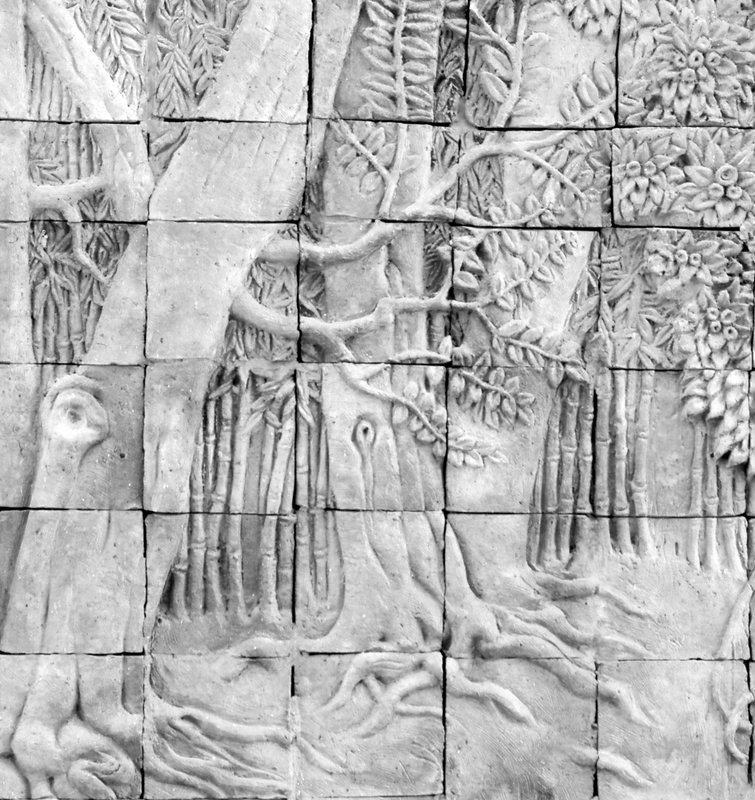
\includegraphics[keepaspectratio, width=2.8cm]{03.jpg}}
\part{Television Interview}

\chapterNote{Conducted by a French television channel.}
\chapter{Interview with Ajahn Vajiro}
% Title: Interview with Ajahn Vajiro
% by a French television channel

\questionBi%
{Comment avez-vous découvert cette tradition des moines de la forêt?}%
{How did you come across the Forest Monk tradition?}

\answer{}
Through an interest in meditation I heard about the Forest Tradition
in 1975. In 1977 I heard that there were Forest Monks in London where I
was living, so I went to see them. They had been invited to stay in
England to live as \emph{bhikkhus}.

\questionBi%
{Vous connaissiez bien Ajan Chah, quel souvenir en gardez-vous?}%
{You knew Ajahn Chah well. What memories do you have of him?}

\answer{}
I cannot claim to have known him well. I did not speak Thai at
all then and never lived with him for a long time.

I met him in 1977 during his first trip outside of Thailand. I was
struck by how at ease he was in whatever situation he found himself in. 
In 1979 he travelled outside Thailand again and I was then part of the
community. He came to check how the community of four monks he had left
in the UK was getting along. At that time someone had offered some
woodland for the forest monks, and a derelict house close to that
woodland had been bought with the funds from selling the property in
London. Ajahn Chah approved of the move, although he could see that the
house was not comfortable. He is reported to have often said that to
begin a monastery is difficult, but easier than to repair and maintain a
monastery, which is more difficult; and finally, that to have good wise
monks living in the monastery is the most difficult. 

I helped with the driving when he was making a tour of the United
Kingdom. We travelled all the way to Edinburgh in a very unsuitable slow
van. He never complained or showed any sign of impatience with the van. 
He did take the opportunity to teach and instruct with economy and
humour. I was drying his bowl, and he came over to where I was and with
the help of one of the other monks translating explained completely all
the stages in taking care of the bowl. And at the end he pointed out, `I
will train you to take care of your bowl, Ajahn Sumedho will teach you
to reach Nibbāna.' In this way he was both teaching me and indirectly
offering something for Ajahn Sumedho, who was within hearing range, 
something to learn from. 

Later when I was already in Thailand, I awaited the occasion to
undertake the full training as a \emph{bhikkhu}. This is called the
ceremony of \emph{upasampadā}. By that time in early 1980, I had been
both a postulant and a novice for longer than almost any foreign to
Thailand person. There were four young novices awaiting the confirmation
of the date. But Ajahn Chah would not give us a date. On a number of
occasions we would go to his monastery from where we were living, all
prepared, all ready, and ask, `When will the ceremony be arranged?' and
he would always just put us off. And then one evening he said, `Go and
prepare the hall, we'll do it tonight.' This was at around five o'clock. 
So we did, and as the evening fell in the tropics in a monastery without
electricity, the ceremony took place. Simple and easy. With no fuss. It
happened to be my birthday. To this day I do not know if Ajahn Chah knew
or, if he did know, whether he thought it at all important. 

\questionBi%
{Revenons maintenant, si vous voulez bien, sur cette tradition des Moines de la Forêt que vous représentez\ldots{} Est-ce que vous pouvez nous rappeler quand elle est née, et dans quelles circonstances\ldots{}?}%
{Please let us come back to this `Forest Monk' Tradition that you represent. Could you remind us when it was born and in what circumstances?}

\answer{}
The Forest Monk tradition is not confined to Thailand and would have
existed in some form from the time of the Lord Buddha.

\questionBi%
{Est-ce qu'on peut définir la particularité de cette tradition?}%
{Can we define the specificities of this tradition?}

\answer{}
The particular branch of the Forest Tradition to which I belong, Wat
Pah Pong, is distinguished by its working as a community. It works
together. It seems to be Ajahn Chah's great offering, the offering of
encouraging people to work together in community. He used the Vinaya, 
the Training in Community, as received from the traditional scriptures, 
and worked out how to allow ordinary people to use that training to
learn to live and work together. 

Often when a great teacher dies the disciples go their own way. You may
have heard that Ajahn Chah was paralyzed and did not speak for about the
last ten years of his life. This was certainly difficult for all of us, 
those who called themselves his disciples. The effect was that we all had
to learn to work together. There were five people nursing him all the
time of his illness. The monks took turns. They had to work together. 

Today the group consists of maybe 1,500 monastics, with about 270
monasteries. Of those monastics, about 150 would not call Thailand their
origin. There are about 20 monasteries not run by Thais which would
look to Wat Pah Pong and that tradition. I think around 17 of
those monasteries are not in Thailand. 

The monasteries vary in size from maybe two monastics, or even one, to
maybe 50. Outside Thailand the largest in number of monastics is
probably Amaravati Buddhist Monastery.\footnote{\href{http://forestsangha.org/monasteries}{www.forestsangha.org/monasteries}}
We all consider ourselves part of this family.

\questionBi%
{Le maître a un rôle très important dans cette tradition\ldots}%
{The teacher has a very important role in this tradition \ldots}

\answer{}
The teacher has an important role, yes. Like the father.

\questionBi%
{Quelles sont les règles qu'un moine de la forêt doit observer?}%
{What are the rules a forest monk should observe?}

\answer{}
There are four which if not observed, automatically, with immediate
effect and without ceremony, disqualify a man from continuing the
training.

\begin{enumerate}
  \item Any sexual intercourse
  \item Theft of something of value
  \item Shortening or causing to be shortened the life of any human.
  \item Lying deliberately to claim that one has attained some special spiritual level.
\end{enumerate}

The particular rule of our tradition and family, which is common to all
Buddhist monks with a connection to the training at the time of the Lord
Buddha, is not to own or control personal money or that which counts as
money.

\questionBi%
{Comment la communauté des moines de la forêt s'est-elle créée puis a-t-elle évolué en Angleterre?}%
{How was the Forest Sangha created in England and how did it develop?}

\answer{}
The Forest Sangha has evolved in the UK through the confidence of and
confidence in the disciples of Ajahn Chah, particularly Ajahn Sumedho. 
He has allowed communities of monastics to grow in the UK. The
confidence has been that if the monastics are living in accordance with
what can be shown to be the teaching of the Lord Buddha, then there will
be enough generosity to support that life. The places where monastics
live in community can be like generators: generators of generosity (they
exist because those who live there are generous in their lives and what
they offer, asking for nothing, and those who support that life are generous
in offering that support of material things); generators of virtue (the
places encourage virtue in those who live there and, through example and
direct teaching, encourage virtue in those who visit); and generators of
an attitude which cultivates reflection or wisdom (they are places where
people meditate, examine their universe from the inside and practise
being enlightened). 

\questionBi%
{Quelles ont été les principales difficultés?}%
{What were the main difficulties?}

\answer{}
The principal difficulty is that of attachment to opinions and views,
and the pain that follows.

\questionBi%
{Vous avez participé, au début des années 80, à l'établissement du monastère d'Amaravati, en Angleterre\ldots{} le premier monastère de forêt en Occident\ldots{} Est-ce que cela n'a pas été trop compliqué? Les réactions ont-elles été favorables?}
{You took part at the beginning of the 80's in the establishment of Amaravati, the first forest monastery in the West. Wasn't that too complicated? Was the public response positive?}

\answer{}
Amaravati was not the first forest monastery, that was Chithurst
Forest Monastery, Cittaviveka.\footnote{\href{http://cittaviveka.org}{www.cittaviveka.org}}

Yes, beginning any monastery is difficult. Not much more difficult in
the West than in the East. A little different. When something a little
out of the ordinary arrives somewhere, there are always a variety of
responses. The main concern seemed to be traffic. Would the place
attract more cars? There were other worries that the strangeness of the
clothing and customs would somehow undermine what was already there. 
Again a clinging to views and opinions. 

\questionBi%
{Quelles sont les grandes différences avec la communauté des moines de la forêt en Thaïlande?}%
{What are the main differences between the Western Sangha and the Thai one?}

\answer{}
The main difference is maybe the timing of the meal. In Thailand it
is long established that the meal is around 08.30 to maybe 09.00, and
that will be the meal for the day. Outside Thailand the meal is usually
a little later, maybe 10, 10.30 or even 11.30. This is because it is
thought that this will make it easier for people to come to the
monastery to be part of that occasion. Of course there are some
differences of dress to accommodate the differences in climate.

\questionBi%
{Les échanges, les liens entre les deux communautés sont-ils aussi forts aujourd'hui?}%
{Are the links between the two communities still as strong today?}

\answer{}
The links nowadays are still strong, almost stronger in the last few
years than they were in the early 80's and mid-80's. Communication is
now a lot less expensive.



\partNote{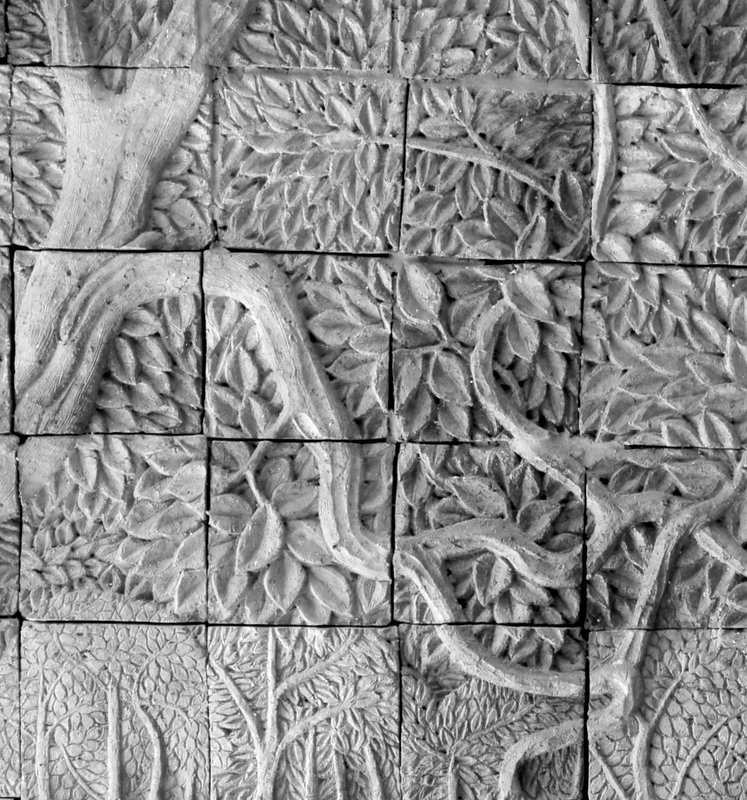
\includegraphics[keepaspectratio, width=2.8cm]{04.jpg}}
\part{A Recent Recollection}

\chapterNote{Recollections by Ajahn Siripañño.}
\chapter[The Luang Por Chah Memorial Week]{The Luang Por Chah\newline \soChapter{Memorial Week}}

\begin{quote}\itshape
Every year during the week leading up to the anniversary of Ajahn
Chah's death on 16\textsuperscript{th} January, there is a great
gathering at his monastery in north-east Thailand, when many of his
disciples come together for six days of Dhamma practice. Ajahn
Siripañño, the senior monk at Wat Dtao Dam at the time of writing, provides the
following account from his perspective of living as a monk in Ajahn
Chah's branch monasteries in Thailand.
\end{quote}

\noindent
12\textsuperscript{th} January 2009, and all over Thailand motorbikes,
cars, pick-up trucks, mini-vans and tour buses are making their way to
the north-eastern province of Ubon, heading for a certain monastery --
Wat Pah Pong. Those making the journey are looking to spend a week
imbibing the spirit and teachings of a forest master now long gone,
Ajahn Chah. Most never met him in person, but the books, tapes and
first-hand accounts of his life have inspired them enough to make changes
in their lives, to take up meditation, and now to join the annual
pilgrimage to where it all began and take part in a week of communal
Dhamma practice. 

The name of the event translates as `Dhamma practice festival in honour
of the Teacher'. Actually, the word \emph{ngan} -- here translated as
`festival' -- usually means work. But it can also mean any kind of event
or celebration: birthdays, weddings, funerals, festivals -- any kind of
activity, really. The Ajahn Chah \emph{ngan} combines many things: the
serious spiritual work of keeping precepts, meditating and listening to
Dhamma talks, socializing with old friends, and having fun making new
ones\ldots{}. This is against the backdrop of reaffirming one's
dedication to living in line with the teachings of the Lord Buddha and, 
more recently, Ajahn Chah, or Luang Por (`venerable father') as he is
affectionately known. Of the thousands who arrive from near and far, 
some come to practise and hear the Dhamma, some to give and participate
in large measure or small, and some come just to check out the scene, 
and enjoy the free food available for all. 

Luang Por Chah passed away on 16\textsuperscript{th} January 1992, and every year since
his funeral on that date the following year, a gathering has taken place
at his monastery Wat Pah Pong. The number of participants keeps
increasing. This year saw over a thousand monks and novices and five
thousand laypeople put up mosquito nets (and, more and more these days, 
tents) all over the monastery, doing their best to let go of the outside
world and focus their hearts on a different dimension. With Luang Por's
teachings as the conduit, the practice turns one inwards -- to taste
peace, know truth and find oneself. 

Tan Ajahn Liem, the abbot of Wat Pah Pong (and these days himself
referred to as `Luang Por') is sitting under his \emph{kuṭī} receiving
some monks as they arrive to pay their respects. A man of few words, he
gives the young monks advice and encouragement like a warm father. `It
just got a bit colder, but it's not too bad. Last night was about 15
degrees. It'll take a couple of days for the body to adjust, that's all. 
If you put your sleeping sheet directly on the hay it will be warmer. A
plastic groundsheet will stop your body heat from getting trapped in the
hollow stalks, so you'll be colder. We have plenty of toilets these
days, so you should be comfortable \ldots{} not like before. There's
space to put up your mosquito nets behind the Uposatha Hall. Around the
\emph{chedi} is full of laypeople these days, so it's not so
appropriate. How many of you came? For the next few days you should
surrender to the schedule. This will help eradicate unwholesome states
of mind such as arrogance and conceit, and the need to have things your
own way. Otherwise you will always fall under the sway of defilements
and craving. It takes effort, though -- \emph{viriyena dukkhamacceti}: 
``suffering is overcome through effort''. But if you practise correctly
your hearts will experience the happiness of inner peace.'

He pauses and looks up. `Have you set up your bowls for the meal yet? 
No? Off you go then. It's almost time.'

The monks and novices head for the eating hall, directly behind the main
\emph{sāla} which is now slowly filling with white-clothed laypeople. 
Women far outnumber men. Before the meal every day the Eight Precepts
are given and there is a half-hour Dhamma talk. On this, the first day, 
it is Luang Por Liem, like a welcoming host, who gives the introductory
talk. He stresses that initially we have come out of faith in the Buddha
and Luang Por Chah, but that in order to carry out their teachings we
need to develop true \emph{sati} -- true mindfulness: 

`We are all just part of nature: the body must change and return to its
origins. When we think in this way the mind will tend to seclusion, 
rather than clinging to views and conceit. Dwelling secluded in body and
mind, we are able to see the true nature of reality. And so we won't
fall under the sway of things that can obsess the mind and wrong views
which stain the mind. The body is just a natural resource we can make
use of -- not a being, not a person, animal or individual. If we
understand this the mind will feel cool and happy, not anxious and
confused. If we strive in this way we will attain the goal we are
seeking. We have a good opportunity, so try to do it: renounce and
abandon the things that cause you worry. The Buddha taught us to abandon
all worldly dhammas. We can't even depend on our friends and relatives. 
Ultimately we have to build our own inner refuge.'

He outlines the daily routine, emphasizing the need to be harmonious and
helpful as we will be spending a week living together in such large
numbers. Meditation, too, is taught in brief.

`Breathe in and out. See that it's just nature doing its job, breath
coming in and going out. When we understand that our awareness of this
is an aspect of our mind, we see that even this is a
\emph{saṅkhata dhamma} (a conditioned phenomenon). There is no self in
there. The mind experiences the breath. The mind has no physical matter, 
yet that is where \emph{dukkha} arises. All mental states are
impermanent, so develop the quality of patient endurance with regard to
all mental states, good and bad. Usually we get lost in our moods, and
this keeps us away from the correct path of practice \ldots{}

`Whatever posture you are in, you are grounded on the earth. Keep this
deep awareness (Thai: \emph{poo roo}) in mind all the time. This way you
won't think of the body as a self. It will lead to a pure happiness
arising in the mind. Instead of delighting in those things which deceive
us -- things people run to like insects drawn to a flame -- cultivate
faith in the Buddha's awakening \ldots{} Develop yourself internally
with your mind and externally with your actions. You all know the duties
regarding the lodgings and toilets. They are communal property, not
owned by anyone, including the abbot. People who are mindful keep a
place clean and well maintained.'

Knowing it's almost nine o'clock, he concludes, `Now it's time to
provide our bodies with the sustenance we need to carry us through the
next day and night, so I will end there. I wish to express my gladness
that you have all come, and encourage you to make a firm determination
to practise with integrity this week.'

For the rest of the day, monks and laypeople arrive at Wat Pah Pong in a
constant stream. Luang Por Liem receives incoming Sangha members under
his \emph{kuṭī} all day, and by evening he still has not had a chance to
find his own spot in the forest to put up his mosquito net and lay down
a bed of straw like everyone else. He is just slipping away when a monk
approaches him quickly to say that Ajahn Sumedho has arrived to pay
respects.

He returns to his seat, first putting on his robe, and the large group
of Western \emph{bhikkhus}, including Ajahn Sumedho, bows three times. 
The two old friends chat for a while, inquiring after each other's
health, and Luang Por Liem asks about the various branch monasteries in
England. They have known each other for almost 40 years. Practising
together in the old days, travelling on \emph{tudong} and serving their
teacher -- theirs is a lifelong bond, bound up with much mutual warmth
and respect. All over the monastery similar scenes are taking place: 
monks who have spent time together in the past are now meeting again, 
paying respects and catching up, like childhood friends. 

After about half an hour there is a pause and Luang Por Liem, a little
sheepishly, excuses himself. `It will be getting dark soon, I still
haven't put up my net.' There are smiles all round and the visitors
again bow three times. Luang Por Liem disappears into the twilight of
the forest. 

By the evening of the first day, several hundred monks have arrived and
the number of laypeople is over three thousand. There are free food
distribution tents set up -- over a hundred different stalls and
marquees sponsored by individuals, branch monasteries, government
offices and other groups. For the next week, almost round the clock
there will be all kinds of food and drink available for anyone who wants
them. Luang Por Kampan Ṭhitadhammo mentioned this in the talk he gave on
15\textsuperscript{th} January. 

`It's as if the whole country is coming together here. This is the
result of Luang Por's life. Just look at the food tents. It's like a
wholesome cycle of goodness. People come here to hear the Dhamma. Then
they give food to others. Other people come to eat, but in doing so they
get to listen to the Dhamma. Then they in turn want to give.'

Some locals, unable to sponsor a tent for the whole week, simply drive
their pick-up into the monastery with the back full of some kind of
tasty snack. Parking it just inside the monastery gate, they hand out
their offerings to passers-by. In not too long the food is gone and they
drive off, happy to have been a part of the event and to have taken the
family on such a fun outing. 

The local hospitals provide first-aid tents as well as traditional Thai
massage and reflexology for the Sangha members. Last year there was free
dental treatment and this year eye tests and glasses were offered in a
marquee just opposite Luang Por's \emph{chedi}. Over the years the scope
of the gathering has broadened, as well as the range of participants. 
Lay supporters from Abhayagiri monastery in California won the hearts of
everyone when they prepared and served American snacks from a food tent
they set up a few years ago. Professionals and teachers from Bangkok
come and camp around the \emph{chedi}, as well as members of what the
Thais call `\emph{Hi So}' (from the English `high society') -- slang for
the aristocracy and well-heeled elite, who genuinely want to put down
much of the superficiality and stress of modern life and reconnect with
something more meaningful and peaceful. Some tents may be fancier than
others, but everyone keeps the Eight Precepts and most stick diligently
to the schedule -- sharing together in the pre-dawn chill of morning
chanting, queuing for food and toilets and splashing down with a bucket
of cold water to bathe. It is no small matter for some. 

Every year more schoolchildren come in large groups. All wearing white
-- girls camping in one area, boys in another -- they have all the
playful energy of teenagers everywhere. But a genuine sense of respect
and decorum is also there, as if they know that although it's not as
much fun as a usual school trip, somehow it's important, and it's only a
few days after all. 

It's 2.45 a.m. Way too early. But from the high bell tower to the north
of the eating hall, the repetitive striking shatters the stillness. It's
time for morning chanting. You do have a choice, though; you could try
to find an excuse to stay bundled up in a heap of robes on the cosy bed
of straw. You're still a bit weak from that diarrhoea a few days ago, 
your throat seems to hurt a bit -- wouldn't want to get sick on day two
-- with so many monks, no one else would really notice if you weren't
there. But it's useless. Only the previous day, in a talk to the Sangha,
Ajahn Anek had reminded everyone that in Luang Por's time everyone was
at morning chanting, and not all wrapped up in brown shawls and
blankets, either. Then you had to sit with your right shoulder exposed, 
patiently enduring the cold weather and practising \emph{ānāpānasati}
 (mindfulness of breathing). You imagine Luang Por Chah's presence
standing next to where you are lying curled up, looking down
stony-faced: `Eugh! Is this how you practise?' Spitting out some red
betel-nut juice, he turns around and disappears into the void. You don't
really have a choice. 

By 3.05 the \emph{sāla} is nearly full with monks sitting, as is the eating
hall. With the exception of one monk known for his eccentricity who has
crafted himself a Mexican-style poncho, almost no \emph{bhikkhus} are wrapped
in blankets as they were the previous morning. Ajahn Anek's words have
had the desired effect, and the new generation of monks seems keen to
show its fighting spirit. 

The laypeople, who somehow seem to have more enthusiasm for morning
chanting than do the monks, have gathered \emph{en masse}, and the women
-- \emph{mae awks} as they are known in the local dialect -- fill the
\emph{sāla} and flow back out along a wide concrete road. At 3.15 the old
grandfather clock chimes and one of the senior monks rings a bell: 
`\emph{Gra--ahp}' he says over the microphone, Thai for `It's time to
bow and chant.' `\emph{Yo so Bhagavā} \ldots{}' The monk with the
microphone tries to push the pace and raise the pitch, but the massed
ranks of \emph{mae awks} have the strength of numbers and the chanting
stays slow and low. Some find the whole thing tedious; others are filled
with devotion and inspiration. For 45 minutes these ancient Pāli words
and their modern Thai translation are recited line by line, to a
slightly singsong melody that is written only in the hearts of those who
know it and who learned it themselves by listening and following along
from the time they first came to the monastery. 

From 4 until 4.45 there is a period of meditation. Fighting the cold and
fatigue, for many it's nothing but a struggle not to wrap up, fall
asleep, or both. Others seem to have found an equanimity of body and
mind. Seated on the hard granite floor, they embody the peace and wisdom
of the Buddhas; still and silent, aware and knowing, breath going in, 
breath going out. 

By 5 a.m. the monks are setting up the eating hall, sweeping, mopping, 
and putting out tissues, water and spittoons. Next they prepare their
bowls and put on their robes for alms-round. A senior
monk has the microphone and is going through some of the points of
etiquette for alms-round: wearing one's robes properly, walking with
eyes downcast, not swinging the arms and body about, keeping silent, and
many other minor points of practice. Some newly ordained monks and
novices may still be learning all this. Others will have heard it year
in, year out. Yet somehow it has a freshness every time and an immediate
relevance. These minor training rules and the small points of monastic
etiquette, collectively called \emph{kor wat} in Thai, were given huge
importance by Luang Por Chah as the way to begin training the mind: by
letting go of doing things one's own way and being mindful to do things
the prescribed way. The Buddha laid down these principles over 2,500
years ago, and Luang Por knew their value. 

Wat Pah Pong has about a dozen alms routes that wind through the
surrounding villages. But when a thousand or so \emph{bhikkhus} are in need of
some sustenance, it's the nearby town of Warin and the city of Ubon that
provide much of the additionally-required calories. As dawn approaches, 
the monks head out of the monastery gates, each with an alms bowl and
some with two if they are attending a senior \emph{bhikkhu}. Lining the
road to the left, right and directly in front of the gate is a motley
fleet of assorted vehicles: draughty buses and pick-ups and, for the
lucky ones, warm mini-vans. The monks swarm aboard and wait. At an
unseen signal, suddenly engines rev and wheels roll, and the parade of
vehicles heads for various markets and residential areas. When they
arrive at their destination the monks form lines of up to 50 or more
and walk along pre-designated routes. People of all ages line the way
and make their offerings, doing their bit for the \emph{ngan}. The food
is simple but bountiful, and by the end of the alms-round each monk may
have emptied his full bowl up to a dozen or more times: sticky rice, 
boiled eggs, instant noodles, orange drinks, tinned fish, bananas, 
coconut sweets \ldots{} staples of the modern Isan (north-east Thai)
diet woven into this hallowed Isan custom -- offering food to the monks
at dawn. No amount of economic crisis, it seems, can deprive people of
this simple joy. And no matter how often one has taken part in this act
of giving and receiving, it remains a little mysterious, and quite
magical. 

The buses and pick-ups return with the monks and countless baskets
brimming with food. There are still two hours until the Sangha will eat, 
and as they walk past the food tents the novices and young monks glance
enviously at laypeople nibbling away on breakfast snacks. The more
senior monks keep their eyes down, having by now learned that watching
someone else eat while you are cold and hungry makes neither you nor the
other person feel any better. 

Everyone gathers at 8 a.m. in the main \emph{sāla} for the daily taking
of the Precepts. A \emph{desanā} then follows, inevitably covering
familiar ground: our debt of gratitude to Luang Por; the importance of
\emph{sīla} as the basis of happiness and the stepping-stone to
\emph{samādhi} and \emph{pañña}; meditation and the need to see through
the illusory nature of our thoughts and moods, to go beyond desire by
establishing a peaceful mind and taste that special happiness the
Buddhas praised and that Luang Por experienced for himself, doing
everything he could for us to be able to do so as well. 

`Careful not to take too much food; think of all the people still behind
you \ldots{} A purse has been found with some money and keys. If you
think it's yours, come and claim it, but you have to say what colour it
is and how much money is in there \ldots{} Remember not to store food
in your mosquito nets. Ants will come for it -- and you'll be tempted to
eat after midday\ldots{}.'

After the meal, once the Sangha members have washed and dried their
bowls, Luang Por Liem gives a 15 minute exhortation, with speakers
hooked up in both the monks' and nuns' eating halls, encouraging us all
to reflect on our duties as \emph{samaṇas}, recluses who have gone forth
from the household life into homelessness: from cleaning toilets to
realizing Nibbāna and everything in between. 

By 10.30 the sun is filtering through the tall trees and slowly warming
up the forest -- time for most people to have a quick lie-down before
the 1 p.m. gathering for meditation and more Dhamma instruction. These
days the Sangha gathers in the \emph{Uposatha} Hall, or \emph{bot} (a
Thai short form of the Pāli word \emph{uposatha}), the building where
Sangha rituals such as ordinations take place. The \emph{bot} is
jam-packed with monks and the heat and stuffiness build up. Heads begin
to nod, then droop entirely. At 2 p.m. a senior monk gives a talk. A
frequent refrain in these afternoon talks particularly aimed at the
monks is how tough it was living at Wat Pah Pong in the early days. All
requisites, including food, were scarce. You couldn't even pick your own
food, as it was ladled into your bowl for you. There was rarely a sweet
drink in the afternoon, and chores were physically draining, including
hauling water from a well to fill jars for toilets, bathing and
foot-washing. Then there were sweeping, cleaning and general
maintenance. If something was broken you tried to fix it, and if it
couldn't be repaired you went without. Requesting a new one wasn't an
option. But it's the love and respect for Luang Por Chah that come
across most vividly from these elder-most senior monks, as expressed in
a talk from Ajahn Anek.

`Luang Por wished us well from head to toe. Even if our minds didn't
like what he was teaching us, our actions had to comply. We were like
children bathing in a cesspit. Our loving father comes along and says,
`Children, what are you doing that for?' `It's fun.' `Get out. Now!' And
Dad reaches in and pulls us out, and gets water to clean us. And pulling
us out is no easy job. Some Ajahns leave their disciples to wallow in
the cesspit. But Luang Por never did. With just his instruction he was
able to extract poison from our hearts. It was like taking a bitter
medicine which tasted awful, but we knew it would save our lives
\ldots{}

`Luang Por's teaching spread far and wide: Patiently endure. Endure with
patience. Dare to be patient. Dare to endure. \emph{Khantī paramaṃ tapo
tītikkhā:} patient endurance is the supreme incinerator of defilements.
\emph{Khantī,} or patient endurance, is like a fire that no coal or
electricity could ever produce. We chant \emph{tapo ca brahmacariyañca}
-- the austerities of leading the Holy Life. These are the austerities
that can burn up our defilements.

`One aspect of this is the morning and evening chanting \ldots{}
Please give up your own preferences and be present for these activities. 
If during morning chanting there are no monks, but for the meal there
are loads, it feels a bit strange, doesn't it? Between following your
own preferences, or the opinion of society, or the Dhamma -- which is
better? These days notions of personal liberty have so filled people's
minds that they have no room for Dhamma any more. Luang Por is still
with us in spirit. So I ask everyone to please meet together in harmony, 
so that if Luang Por were here in person he would be happy.'

The Sangha pays respects to the senior monk who has given the talk and
an announcement is made to go to the eating hall for the afternoon drink
\ldots{} `if there is one.' It's a slightly tongue-in-cheek reminder
that we shouldn't take anything for granted. These days, though, there
is always something available. Tea, cocoa, freshly squeezed sugarcane
and orange juice; drinks containing aloe vera chunks and other
afternoon-allowable `medicinal' nibbles: sugarcane lumps, candied ginger
and a kind of bitter-sour laxative fruit known as \emph{samor}. The
laypeople too have had their fill of afternoon Dhamma, and those keeping
the Eight Precepts partake of similar fare. 

Everyone is encouraged to take part in a group walking meditation
circumambulation around the \emph{chedi}, the monument to Luang Por Chah
where his crystallized bones, revered by many as holy relics, are kept. 
All too soon it is almost 6 p.m. and the bell is ringing for evening
chanting. The relentlessness of the schedule is a reflection of Luang
Por's training methods: keep everyone pushing against their own
preferences and desires in order to go beyond them; surrender to the
communal routine and allow the sense of self to dissolve into a group
identity; and beyond that to experience the sense of being nothing other
than nature arising and passing away; to have constant reminders and
teachings so that the Dhamma seeps into one's mind -- and the
transformation from being one who suffers through clinging to one who is
free through letting go can take place. 

The first hour of the evening session is silent meditation. The January
air is crisp and cool, and it is the mosquitoes' feeding time. The
\emph{sāla} is full, and all around it and stretching into the forest
are men and women wrapped in white, some young though most older, simply
sitting, being aware of the in- and the out-breath. Inside the
\emph{chedi} too people are meditating, finding warmth in the enclosed
space and inspiration from being so physically close to Luang Por's
remains. As they sit, groups of people, families, children, stream in
and out and pay respects -- three bows -- before heading off, perhaps to
get some noodles at the food tents, or maybe just going home. Over in
the \emph{sāla} the chanting begins, and the voice of the monk leading
it drifts into the \emph{chedi} from a nearby loudspeaker. Many of the
meditators stay motionless, but most slowly open their eyes, and shift
their posture from cross-legged to kneeling in the traditional Thai way
for chanting. By some kind of unvoiced mutual consent they agree that
the monks' pitch is a little too high and settle for something a few
tones lower -- creating an eerie discord which echoes hauntingly around
the inside of the chamber. 

Outside it's noticeably colder. By the time the evening \emph{desanā}
starts at around 8 p.m. the northern wind has picked up, adding to the
talk the flavour of \emph{khantī} -- patient endurance. This was always
one of Luang Por's favourite themes anyway, one reflects. The monks
giving the week's evening talks are Luang Por Chah's most senior
disciples. They know how to inject lightness and humour into their
teachings; stories of Luang Por abound, as well as humorous anecdotes
from their own lives. The language used is mainly central Thai, but
those monks who are native to the north-east will often switch abruptly
to the local Isan dialect, a language full of puns, wordplay and
innuendo, much to the delight of the local crowd. Dhammapada verses, old
sayings, and nearly-forgotten proverbs are given an airing, complete
with the Ajahn's personal commentary. Isan is not a written language, 
and listening to these old monks one gets a sense of the power of an
oral tradition. Even if none of Luang Por's teachings had been recorded, 
we would still be able to enjoy them today from the minds and through
the voices of the disciples he touched. The Buddha's teachings were not
written down for several centuries, yet they managed to survive in a
similar way. 

You are asleep the second your head hits the straw mattress. One day
merges seamlessly into another -- all too soon that monk in the bell
tower is doing his thing and you find yourself heading back to the
\emph{sāla} for morning chanting. Each day is a little easier, though. 
The floor seems less hard. It's a bit warmer, too. The mind is uplifted, 
buoyed by the company of so many people sharing the space and practising
in the same way. Surely that's what it is -- though maybe it's something
else\ldots{}. 

\subsection*{16\textsuperscript{th} January}

The big day arrives. As if to acknowledge one of
the unique aspects of Luang Por's legacy, the international Sangha, the
morning Dhamma talk will be given by Ajahn Jayasāro, who is English. The
evening programme will feature Dhamma talks to be given throughout the
night, but the first one -- the prime-time slot -- will be from Luang
Por Sumedho. 

It is 17 years to the day since Luang Por passed away. He was
cremated on the same day one year later. The main event of the day is a
mass circumambulation of the \emph{chedi} by the whole assembly. The
numbers will swell to many hundreds more, boosted by people who have
come just for this event. With the whole Sangha and all the laypeople
gathered together like a sea of brown robes followed by a white foamy
wake, the effect is quite magical. Beginning in the main \emph{sāla}, 
the assembly walks in complete silence, everyone holding a small set of
candles, flowers and incense, for the few hundred metres until the
\emph{chedi}, which the procession then circumambulates. As everyone
gathers round the \emph{chedi}, a senior monk reads out a dedication to
Luang Por and everyone follows, reciting line by line. The Sangha leads
the way up the steps and into the \emph{chedi}. Each person places their
little offering, then bows and makes way for someone else. 

In the evening Luang Por Sumedho begins his \emph{desanā}. Before moving
to loftier dhammas, he too entertains the crowd with some warm old
memories. He recalls how Luang Por used to teach the Dhamma for hours on
end, cracking jokes and telling stories which would have everyone in
stitches -- except for one person: Venerable Sumedho, this newly arrived
American monk squirming in pain on the cement floor, unable to
understand a word. They've heard it before, but again it brings smiles. 
These stories though, are not told just to get a few laughs. They
capture the spirit of a bygone era for those of us who never heard Luang
Por Chah teach, and they prepare the minds of the listeners to hear and
be more likely to truly receive the essence of the Dhamma: that all is
uncertain and unstable, and that happiness comes from letting go. 

Which is just the insight you need in order to last through a whole
night of Dhamma talks. This all-night talks routine seems to be a unique
feature of the Wat Pah Pong tradition -- and you have to be seriously
dedicated to hearing Dhamma to even want, let alone be able, to sit on a
hard floor for ten hours. Understanding the language, too, is a distinct
advantage. Most people nip off for a small rest at some point in the
evening; but some seem to sit motionless throughout, in a kind of
`\emph{desanā} trance'. The first couple of speakers talk for about an
hour; after that it's half an hour each. So, altogether 15 or so
Dhamma talks ring throughout the forest on loudspeakers right through
till dawn. A bell is struck to let any speaker who's getting a bit
carried away know that his 30 minutes are up. The style of \emph{desanā}
is usually unstructured, which is typical of the Thai forest tradition. 
Anyone who miscalculates his allotted time can therefore easily wrap up
and make way for the next speaker when he hears the bell. The last
speaker is still going at full speed at 5 a.m. as the monks, for one
last time, begin to set up the eating hall and then stream out through the gates
towards the waiting armada of alms-round road transport. 

On this last morning the Sangha and laity gather in the \emph{sāla} one
final time, to take leave and ask forgiveness of the most senior monks. 
After a week of remembrance dedicated to Luang Por Chah, it seems
fitting that the endnote is an acknowledgement of our present-day
teachers. Luang Por Liem, appointed by Luang Por Chah to be his
successor as abbot of Wat Pah Pong, receives the traditional offerings
of tooth-woods -- wooden toothbrushes made from a bitter vine that the
monks meticulously fashion in advance and bring to the gathering to give
to senior Ajahns as a token of respect. 

After a few words of farewell and one last blessing the 2009 memorial
gathering is over. The last meal is taken and followed by a mass exodus. 
Thousands of mosquito nets are taken down and tents dismantled; vans are
loaded, with as many as 15 people crammed in to the back of a
pick-up truck for journeys of up to several hundred kilometres. Rubbish
is collected and areas swept. In the eating hall the spittoons are dried
one last time, the water bottles bagged up for recycling, the sitting
mats put away. Within a few hours the monastery feels deserted. Only the
resident community of 40 or so monks and the nuns in their own
section remain, doing the final clear up. 

The following day is a Sunday. In the afternoon some visitors, including
a couple from Bangkok, stop by Wat Pah Pong to pay respects, and
hopefully make some offerings to Luang Por Liem. A lone monk sweeps the
concrete road around the \emph{chedi}, and not a trace remains of the
thousands of residents over the previous week or the mass
circumambulation the day before. Not someone who seems too interested in
taking a break after a hard day's night, Luang Por Liem is in town
looking for building materials. He won't be long, though, the group is
told. Sure enough, within half an hour he is back. `I went into town to
get some pipes. We are building more toilets for next year's gathering. 
More and more people seem to come. More people means more waste. It's
natural. If we can see the body as part of nature -- natural elements
and not a self -- then peace will arise in the heart. This peace leads
to true happiness.'

\subsection*{Extracts from a desanā given by Ajahn Jayasāro}

It's been 17 years now since Luang Por left us, although actually
that is not quite true. Luang Por never left us -- we are the ones who
leave him behind. Every time we think, say, or do something of which he
pointed out the danger, we leave him behind. There are so many of his
teachings around: books, tapes etc. His Dhamma is still with us. But we
frequently leave his teachings behind, sometimes turning our backs on
the Dhamma entirely. Luang Por Chah is not with us today, but the
question is, are we still with Luang Por Chah? 

\ldots{} Not having Right Understanding (\emph{sammā diṭṭhi}) is what
will prevent true happiness from arising. We won't see the true nature
of the world: the fact that \emph{dukkha} is everywhere. The good news
is that true happiness can also be found. It is not about suppressing
the happiness that we can experience through the eye, ear, nose, tongue, 
body and mind, but rather asking ourselves if that is true happiness. Is
that what we ultimately need ? Sensory happiness makes us waste our time, 
and diverts our interest away from developing ourselves to find that
true happiness. 

Say you had enough money to go abroad and you flew to some other
country. Then from the airport you went straight to a hotel, checked in
and went to your room, closed the windows and stayed there for two
weeks. You then went back to the airport and flew home. Would that be
unwholesome? No. But it would be a pity, a wasted opportunity. Being
born as a human being, but only being interested in the pleasure of
sights, sounds, smells, tastes, touch and thoughts, is a similar waste. 
It's really like living in a dark room. 

\ldots{} Luang Por Chah taught us that our real task in life is to
cultivate a healthy shame and fear of losing our mindfulness
(\emph{sati}). We must always strive to maintain \emph{sati}. If we have
\emph{sati}, it's like we have an Ajahn with us. We feel warm and safe:
whenever we make our mind steady, wisdom is ready to arise. Without
\emph{sati} we will always be slaves of our environment and simply
follow whatever thoughts and moods arise.

\subsection*{Extracts from an 8 a.m. \emph{desanā} given by Luang Por Bundit}

Every second our thoughts and moods are teaching us. People without
Right Understanding think, `Why is it so hot?' or `Why is it so cold?'
But it's just nature doing its job. We don't have to make such a big
deal out of it. If we don't understand the world, we will always
experience \emph{dukkha}. Disappointments will be difficult to accept
and we'll always be living for our hopes and dreams. 

\ldots{} People used to come to pay respects to Luang Por Chah, and
would complain they didn't have time to practise, that they were too
busy looking after their children and everything else. `Do you have time
to breathe?' he would ask. `Yes.' `Well then, practise like that!'

Take up the five primary meditation objects that preceptors give the
newly-ordained as a theme for contemplation: hair of the head, hair of
the body, nails, teeth and skin. Doing this will help free us from being
slaves to the body and all the usual concerns regarding beautification
and health, and obsession with treatments and therapy. 

Luang Por taught us to abandon everything. He repeated it again and
again. In the old days there were no doubts about the correct practice, 
but now everyone has a different opinion about Luang Por's teachings. 

So learn to choose the pure things in life. If you know those things
which are pure and lead to peace, then you will bear witness to the
truth yourself. No one can do it for you, or verify the fruit of your
practice. It's \emph{paccattaṃ} -- to be experienced individually. 

Well, that is enough for today, I'm sure everyone is very hungry. Learn
to choose Dhamma teachings the way you choose the fish you eat. A fish
has scales, bones, intestines, and flesh. Whether you choose the flesh
is up to you. 



\emptypage

%% Backmatter
%% ==========
%% Glossary, Notes, Index...

\backmatter

\bookmarksetup{startatroot}

%% Copyright details
%% -----------------

\cleartorecto
\thispagestyle{plain}

\vspace*{-2\onelineskip}
\enlargethispage{\onelineskip}

{\smaller\setlength{\parindent}{0pt}%
\raggedright\label{copyright-details}
\setlength{\parskip}{5pt}
{\centering

{\large\ccbyncnd}

This work is licensed under a Creative Commons\\
Attribution-NonCommercial-NoDerivs 3.0 Unported Licence.\\
\href{http://creativecommons.org/licenses/by-nc-nd/3.0/}{http://creativecommons.org/licenses/by-nc-nd/3.0/}

}

You are free:

\begin{packeditemize}
\item to copy, distribute, display and perform the work
\end{packeditemize}

Under the following conditions:

\begin{packeditemize}
\item Attribution: You must give the original author credit.
\item Non-Commercial: You may not use this work for commercial purposes.
\item No Derivative Works: You may not alter, transform, or build upon this work.
\end{packeditemize}

With the understanding that:

\begin{packeditemize}
\item Waiver: Any of the above conditions can be waived if you get permission from the copyright holder.
\item Public Domain: Where the work or any of its elements is in the public domain under applicable law, that status is in no way affected by the licence.
\item Other Rights: In no way are any of the following rights affected by the licence:
\begin{packeditemize}
\item Your fair dealing or fair use rights, or other applicable copyright exceptions and limitations;
\item The author's moral rights;
\item Rights other persons may have either in the work itself or in how the work is used, such as publicity or privacy rights.
\end{packeditemize}
\item Notice: For any reuse or distribution, you must make clear to others the licence terms of this work.
\end{packeditemize}

Amaravati Publications asserts its moral right to be identified as the
author of this book.

Amaravati Publications requests that you attribute ownership of the work
to Amaravati Publications on copying, distribution, display or
performance of the work.

If you are interested in translating this text into another language,
contact us for formatting guidelines, text material, and help with
copyright issues on the addresses given at the front.

}


\clearpage
\thispagestyle{empty}
\mbox{}

\end{document}
